
%<*discreteCounting.intro>
%<*discreteCounting.Title>
\chapter{Foundations of Counting}\label{chap1}
%%%%%%%%%%%%%%%%%%%%%%%%%%%%%%%%%%%%%%%%
%%%%%%%%%  New Section  %%%%%%%%%%%%%%%%
%%%%%%%%%%%%%%%%%%%%%%%%%%%%%%%%%%%%%%%%
\setcounter{section}{-1}
\section{Mathematical Outcome}

%<*discreteCounting.mathOut1a1>
Activity~{\normalfont\ref{careful}} focuses on developing a method to quickly count large numbers of related objects. This method of counting is called the Fundamental Counting Principle\index{Fundamental Counting Principle}. Before we describe this principle we must first define necessary terminology.
\begin{definition}
Two events are \textbf{independent}\index{independent event} if the occurrence of a particular outcome for the first event does not make the outcomes in the second event any more or less likely to occur.
\end{definition}

%</logic.intro3>
%<*discreteCounting.intro2>
%<*counting.intro1>
For example, if the number of chairs in a house is one event and the number of houses in the street is the other event, then these events are independent. In other words, as long as the number of possible outcomes of event $2$ does not change after you choose an outcome from event $1$, your events are independent\index{independent event}. When making a choice in one event changes the number of possible outcomes in another event, we say these events are dependent\index{dependent}.

\begin{definition}
The \textbf{Fundamental Counting Principle}\index{Fundamental Counting Principle} is the method of counting the number of ways to sequentially choose $x$ outcomes, each one coming from one of a sequence\index{sequence} (a list that has an order) of $s$ independent events. If event $i$ has $n_i$ possible outcomes then the number of different choices of $x$ outcomes is the product $n_1\times n_2\times \cdots \times n_x$.
\end{definition}
% In Activity~{\normalfont\ref{fundprinc}}, we call these events categories and the outcomes are objects. 
Through the students' work in Activity~{\normalfont\ref{whatif}}, they should notice that there are situations where the Fundamental Counting Principle\index{Fundamental Counting Principle} is not applicable. As is suggested in the definition, the Fundamental Counting Principle will work only if the events are independent\index{independent event}. 

We will refer to the occurrence of choosing a single outcome from each event as an option. There are at least two distinct ways of counting the number of outcomes in each question from Activity~{\normalfont\ref{careful}}. One may most naturally use either multiplication or repeated addition to accomplish this task. Both are acceptable methods. Say one has $2$ independent\index{independent event} events where event $1$ has $n_1$ options and event $2$ has $n_2$ options. Then there are $n_1\times n_2$ different outcomes. The other way to find the number of different outcomes is to say you have $n_1$ options in event $1$ for each of the $n_2$ options in event $2$. So there are $$\underbrace{n_1+n_1+\cdots+n_1}_{\text{$n_2$ times}}$$ 
total outcomes. These counting methods are useful for calculating recursions\index{recursion} as well as for pattern recognition.

There are many tools that can be used to systematically count the number of options in Activity~{\normalfont\ref{fundprinc}}. One such tool is the tree diagram\index{tree diagram} seen in Questions~{\normalfont\ref{systematic}} and {\normalfont\ref{systematic2}} from Activity~{\normalfont\ref{careful}}.
\begin{definition}
A \textbf{tree diagram}\index{tree diagram} is a tool used to systematically list all outcomes when choices are being made sequentially. 
\end{definition}
In this chapter, our trees start with ``Customer Arrives'' so as to be more understandable to the problem at hand. Then at each subsequent step in the sequence\index{sequence}, branches are drawn from each vertex in the previous level, each such branch listing one of the possible options based on the choices made so far.

%</discreteCounting.mathOut1a1>
Figure~{\normalfont\ref{sysPic}} is one such example of a tree diagram\index{tree diagram}.
%<*discreteCounting.mathOut1a2>
Trees are a useful tool to form a systematic list of all the outcomes of an event, making it simpler to avoid missing any of the outcomes. Counting using the tree structure can be applied to both independent\index{independent event} or dependent\index{dependent} events, so we can use trees in all discussions on counting. The only downside is that if you have a lot of outcomes for the first event and a lot of outcomes for the second event, then already the tree may be too big to manage. Even so, trees are excellent method to further students' understanding of the Fundamental Counting Principle\index{Fundamental Counting Principle}.

When counting the number of options in Activity~{\normalfont\ref{whatif}}, the Fundamental Counting Principle cannot be used directly because these are dependent\index{dependent} events. However, one may use the Fundamental Counting Principle\index{Fundamental Counting Principle} developed in Activity~{\normalfont\ref{careful}} and then subtract (or add) the unwanted (the missing) options. 

While we will not formally develop the idea of permutations and combinations, the arrangement of all the combination\index{combination} numbers into a triangular array such that the $n^{th}$ row (starting with $n=0$) contains all the choose numbers $\binom{n}{i}$ for all $i$ between $0$ and $n$ is accredited to the French mathematician Blaise Pascal (although other mathematicians were using this arrangement well before Pascal). Hence the name Pascal's triangle\index{Pascal's triangle}. This arrangement of numbers allows us to recognize many relationships between the combination\index{combination} numbers.

\renewcommand{\thefigure}{\arabic{chapter}.\arabic{figure}(\alph{bluefigure})} 
 \setcounter{bluefigure}{1}
\addtocounter{figure}{-1}
%\addtocounter{bluefigure}{1}
\begin{figure}[htb]
\begin{center}
%\includegraphics[width=2in]{}
\end{center}
\[
\begin{array}{cc}
\text{Row number} & \\
0 & 1 \\
1 & 1\;\;\;\;1 \\
2 & 1\;\;\;\;2\;\;\;\;1\\
3 & 1\;\;\;\;3\;\;\;\;3\;\;\;\;1\\
4 & 1\;\;\;\;4\;\;\;\;6\;\;\;\;4\;\;\;\;1 \\
5 & 1\;\;\;\;5\;\;\;10\;\;\;10\;\;\;5\;\;\;\;1 \\
\end{array}
\]
\caption{First six rows of Pascal's triangle\index{Pascal's triangle}}\label{pascaltriangle}
\end{figure}

% \textbf{Constructing Pascal's Triangle.}
We begin with the first row as the single number $\binom{0}{0} = 0!=1$. 
% Some may take issue with $0!=1$ at first, but if one thinks about how many ways you can choose 0 objects from a collection of 0 objects, it makes since to do nothing and there is only one way to do nothing!
One can simply regard it as a definition; it turns out to be useful in that it fits the purpose in formulas in which it plays a role.
Now the second row consists of the two numbers: $\binom{1}{0} = 1$ (there is only one way to choose no objects) and $\binom{1}{1}=1$. We continue this indefinitely placing in the $n^{th}$ row the numbers $\binom{n}{0},\binom{n}{1},\binom{n}{2},\ldots,\binom{n}{n}$ from left to right as in Figure~{\normalfont\ref{pascaltriangle}}.

In this arrangement it is easy to see the symmetry of the triangle. If we draw a vertical line down the center of the triangle we see that each number to the left of the line also appears on the right of the line. To explain why this is true we asks the students to think about $\binom{n}{r}$ versus $\binom{n}{n-r}$ in Question~{\normalfont\ref{3outof10}} of Activity~{\normalfont\ref{Selecting a Jury}}. There are many other patterns mathematicians study inside Pascal's triangle but the depth of that study is beyond the scope of this book.


\newpage
\wbnewpage

%%%%%%%%%%%%%%%%%%%%%%%%%%%%%%%%%%%%%%%%
%%%%%%%%%  New Section  %%%%%%%%%%%%%%%%
%%%%%%%%%%%%%%%%%%%%%%%%%%%%%%%%%%%%%%%%

\section{Activity: Ice Cream Parlor}\label{fundprinc}

\subsection{Entrance Activity: Jack's Ice Cream Parlor}\label{careful}

\Instr{  
Goals for this activity:
\begin{packedItem}
\item Using tree diagrams as a viable counting method;
\item collecting data for developing abstract conjectures; and
\item developing the Fundamental Counting Principle for independent events.
\end{packedItem}
}

%<*chap1:fundprinc:careful:intro2>
Jack's famous ice cream shack serves only two flavors (vanilla and chocolate) and offers only one cone type (sugar). Jack's ice cream shack was suddenly inundated with customers, so to save time a customer must choose either one scoop or two scoops of a single flavor of ice cream. (So no mixing of flavors is allowed. This restriction applies throughout all of Activity~{\normalfont\ref{careful}} and {\normalfont\ref{Nomix}}.) 
%</chap1:fundprinc:careful:intro2>
\begin{enumerate}
%<*chap1:fundprinc:careful:family>
\item A family of five enters Jack's shop. All five hope to place different orders. Is this possible? Find a systematic way to list all the different possible orders.
%</chap1:fundprinc:careful:family>

\Instr{  Start this activity with a round table discussion on what the definition of ``different'' exactly means for this problem. Ask the students some questions related to this topic.

Once that is accomplished, let them continue solving the problem. The list of all possible orders is $1$ scoop of chocolate on a sugar cone, $2$ scoops of chocolate on a sugar cone, $1$ scoop of vanilla on a sugar cone, and $2$ scoops of vanilla on a sugar cone. So there are $4$ different orders.
Therefore it is not possible for everyone in the family to place a different order.}

\wbvfill

%<*chap1:fundprinc:careful:systematic>
\item\label{systematic} Jack suddenly becomes generous and allows customers to choose up to three scoops of a single flavor of ice cream. How many different orders can be made? Find a systematic way to list all the different orders.
%</chap1:fundprinc:careful:systematic>

\Instr{  
Now there are $6$ choices and each family member can have a unique ice cream order. To attain this number the students may approach this question in many different ways. One approach would be to make a table, perhaps with two columns headed by the flavors vanilla and chocolate. 
\begin{center}
\begin{tabular}{|c|c|}
\hline
Vanilla & Chocolate \\
\hline
$1$ scoop & $1$ scoop \\
$2$ scoops & $2$ scoops \\
$3$ scoops & $3$ scoops \\
\hline
\end{tabular}
\end{center}
It will be important for the students to develop the methodology of tree diagrams, as these are one of the best tools for the larger and more complex problems seen later in this activity. Trees also give a visual description of the \textbf{Fundamental Counting Principle}\index{Fundamental Counting Principle}. Figure~{\normalfont\ref{sysPic}} is an example of how to organize the information in this problem using  a tree diagram\index{tree diagram}.
\renewcommand{\thefigure}{\arabic{chapter}.\arabic{figure}(\alph{bluefigure})} 
 \setcounter{bluefigure}{1}
\addtocounter{figure}{-1}
%\addtocounter{bluefigure}{1}
\begin{figure}[htb]
\begin{center}
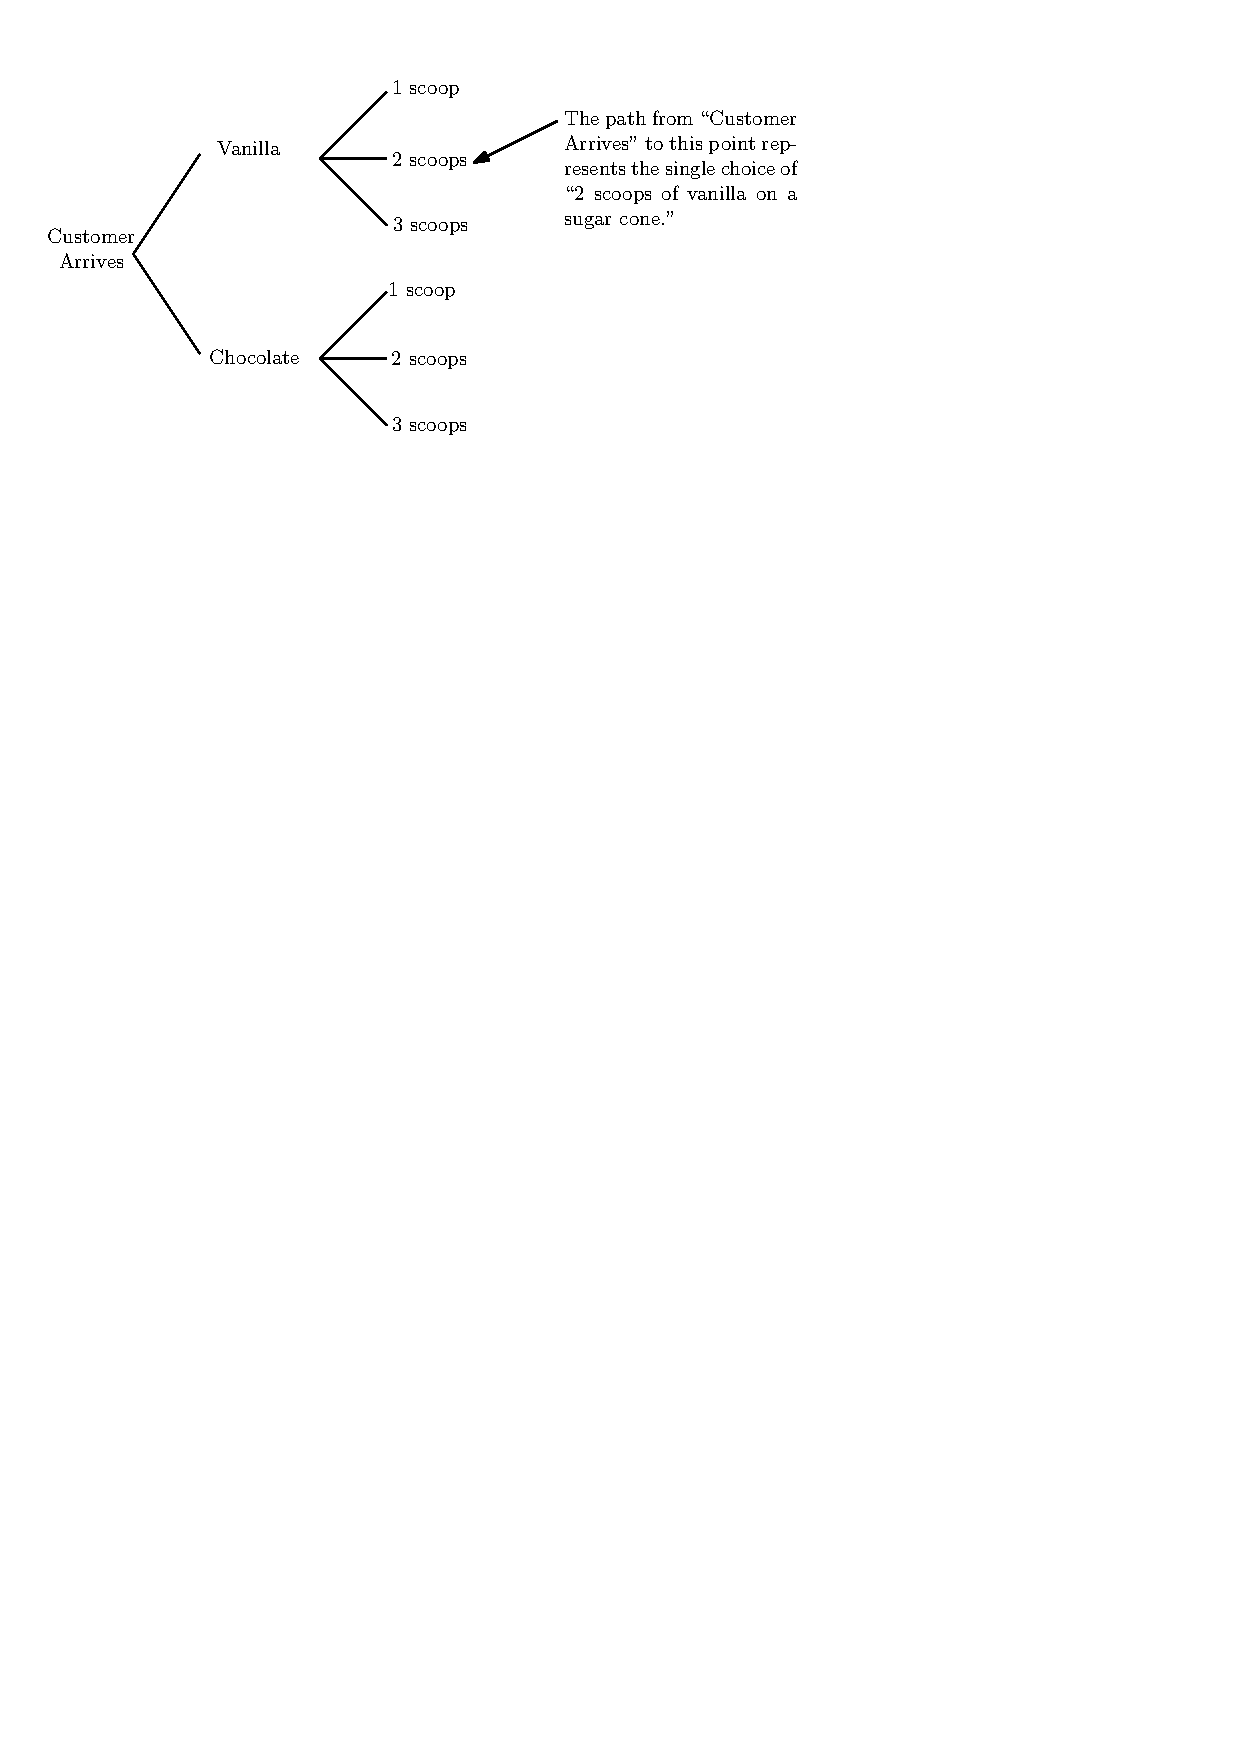
\includegraphics[width=4.2in]{images/tree.pdf}
\end{center}
\caption{Tree diagram\index{tree diagram} of Question~{\normalfont\ref{systematic}}} 
\label{sysPic}
\end{figure}

\noindent It may take some time to get the students used to reading a tree. Encourage them to ``walk'' from ``Customer Arrives'' along edges until you get to the end of a branch; that entire walk yields one order of ice cream. They may also prefer to use the tree in Figure~{\normalfont\ref{systematicPicAlt}} which is also a correct method.
\renewcommand{\thefigure}{\arabic{chapter}.\arabic{figure}(\alph{bluefigure})} 
% \setcounter{bluefigure}{1}
\addtocounter{figure}{-1}
\addtocounter{bluefigure}{1}
\begin{figure}[htb]
\begin{center}
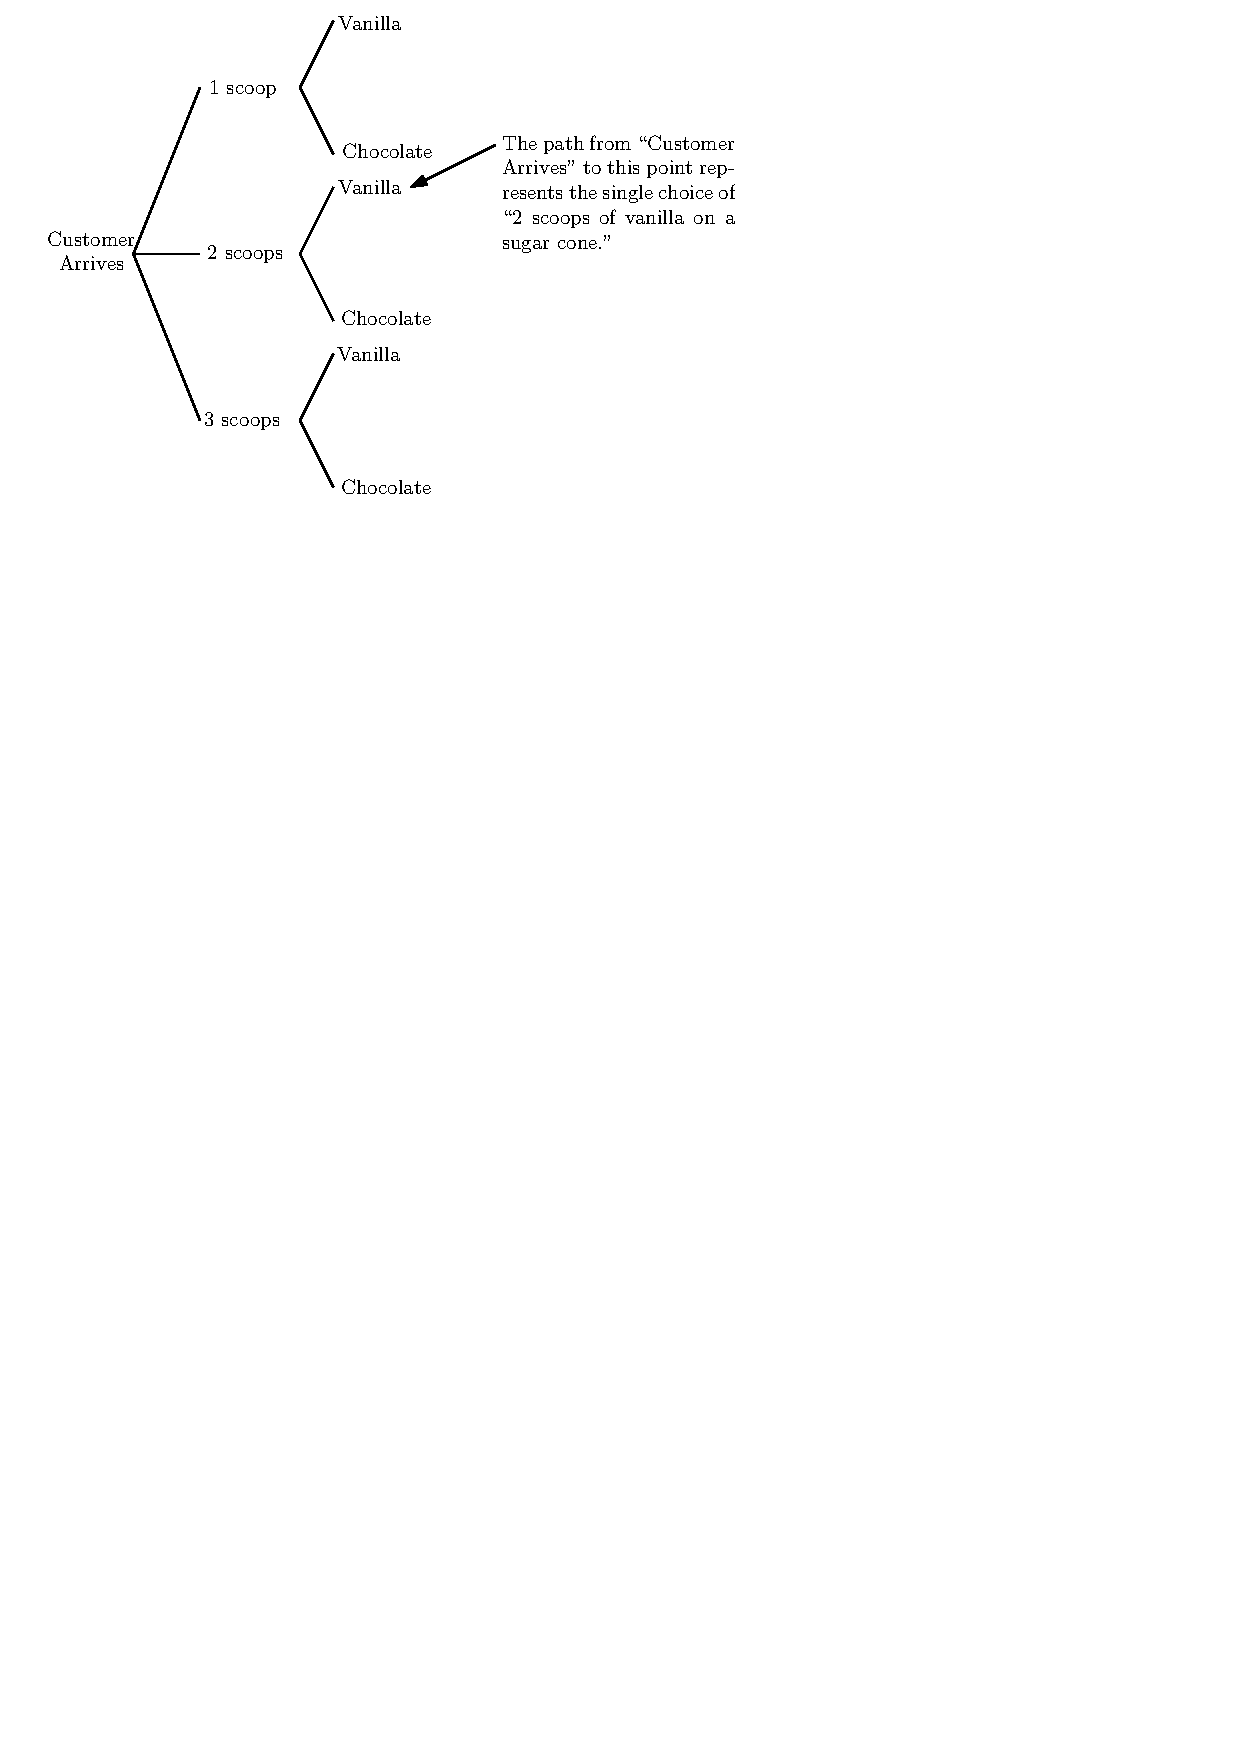
\includegraphics[width=3.6in]{images/treeAlt.pdf}
\end{center}
\caption{Alternative tree diagram\index{tree diagram} of Question~{\normalfont\ref{systematic} }}
\label{systematicPicAlt}

\end{figure}

\noindent In this activity the flavor of ice cream is mentioned first in most questions to ensure students do not think they can mix flavors on a cone: for example they \underline{cannot} have chocolate ice cream on the first scoop and vanilla on the second scoop (we discuss such types of problems in Activity~{\normalfont\ref{whatif}}).
}
\end{enumerate}

\wbvfill

 \newpage


%%%%%%%%%  New SubSection  %%%%%%%%%%%%%%%%

\subsection{ Activity: No Mixing Flavors Allowed}\label{Nomix}

Jack's famous ice cream shack served only two flavors (vanilla and chocolate) and offers only one cone type (sugar). To expand costumer choice, he add a third flavor of strawberry ice cream. Customer must choose either one scoop or two scoops of a single flavor of ice cream. (So no mixing of flavors is allowed. This restriction applies throughout all of Activity~{\normalfont\ref{careful}} and {\normalfont\ref{Nomix}}.) 

\begin{enumerate}

%<*chap1:fundprinc:careful:secret>
\item\label{secret} If Jack allows up to two scoops of one of the three flavors (no mixing of flavors on a cone is allowed!), how many different orders can be made?
%</chap1:fundprinc:careful:secret>

\Instr{  There are $2\times 3=6$ different possible orders. Notice that choosing the number of scoops has no affect on the flavor chosen. If the occurrence of a particular outcome for one event (the number of scoops) does not make the outcomes in the second event (flavor of ice cream) any more or less likely to occur this these two events are said to be \textbf{independent}\index{independent} of each other. It is useful to determine if when several outcomes are independent since the Fundamental Counting Principle\index{Fundamental Counting Principle} may be applied in such situations.
The \textbf{Fundamental Counting Principle}\index{Fundamental Counting Principle} is the method of counting the number of ways to sequentially choose $x$ outcomes, each one coming from one of a sequence\index{sequence} (a list that has an order) of $s$ independent events. If event $i$ has $n_i$ possible outcomes then the number of different choices of $x$ outcomes is the product $n_1\times n_2\times \cdots \times n_x$.
}% ordersper.}

\wbvfill

%<*chap1:fundprinc:careful:sfctable>
\item\label{sfctable} Jack decided to always have up to $2$ scoops and just one type of cone, but made more flavors available. Complete the table below by finding the number of different possible orders in each case. Mixing of flavors on the cone is still not allowed. (You already know the answer for the first two rows.)
\begin{table}[H]
\begin{center}
\begin{tabular}{|c|c|c||c|}
\hline
Maximum number & Number of & Number of & Number of \\
of scoops & flavors available & types of cones & different orders \\
\hline
\hline
$2$ & $2$ & $1$ & \\
\hline
$2$ & $3$ & $1$ & \\
\hline
$2$ & $4$ & $1$ & \\
\hline
$2$ & $5$ & $1$ & \\
\hline
$2$ & $f$ & $1$ & \\
\hline
\end{tabular}
\end{center}
%\caption{Number of different possible orders based on the number of scoops, flavors, and cone types available}\label{sfctableActual}
\end{table}
%</chap1:fundprinc:careful:sfctable>

\Instr{  
Table~{\normalfont\ref{sfctable2}} gives the number of different orders depending on the number of flavors.
\renewcommand{\thetable}{\arabic{chapter}.\arabic{table}(\alph{bluetable})} 
 \setcounter{bluetable}{1}
\addtocounter{table}{-1}
%\addtocounter{bluetable}{1}
\begin{table}[htb]
\begin{center}
\begin{tabular}{|c|c|c||c|}
\hline
Maximum number & Number of & Number of & Number of \\
of scoops & flavors available & types of cones & different orders \\
\hline
\hline
$2$ & $2$ & $1$ & $4$ \\
\hline
$2$ & $3$ & $1$ & $6$ \\
\hline
$2$ & $4$ & $1$ & $8$ \\
\hline
$2$ & $5$ & $1$ & $10$ \\
\hline
$2$ & $f$ & $1$ & $2f$ \\
\hline
\end{tabular}
\end{center}
\caption{Number of different orders based on the number of scoops, flavors, and cone types available}\label{sfctable2}
\end{table}

You may want to ask the students

\begin{minipage}[H]{5.75in}
\tt \em
\begin{center}
{``Why is there a column for the number of types of cones?''}
\end{center}
\end{minipage}

The goal is to get the students to realize we only have one cone type at this point but this may change in the future. The students may also realize that because the number of cone types is $1$, each possible ice cream order must include the same cone type.
}

%<*chap1:fundprinc:careful:sfctable2>
\item\label{sfctableTable} Now suppose Jack allows up to $3$ scoops but still just one type of cone. Complete the table below by finding the number of different orders for the various numbers of flavors; mixing of flavors on the cone is not allowed. (You already know the answer for the first row.)

\begin{table}[htb]
\begin{center}
\begin{tabular}{|c|c|c||c|}
\hline
Maximum number & Number of & Number of & Number of \\
of scoops & flavors available & types of cones & different orders \\
\hline
\hline
$3$ & $2$ & $1$ & \\
\hline
$3$ & $3$ & $1$ & \\
\hline
$3$ & $4$ & $1$ & \\
\hline
$3$ & $5$ & $1$ & \\
\hline
$3$ & $f$ & $1$ & \\
\hline
\end{tabular}
\end{center}
%\caption{Table for Question~{\normalfont\ref{sfctableTable}}}\label{sfctable2table}
\end{table}
%</chap1:fundprinc:careful:sfctable2>

\Instr{  
Table~{\normalfont\ref{numDiffOrderTable}} gives the number of different orders based on the number of scoops, flavors, and cone types available.
\renewcommand{\thetable}{\arabic{chapter}.\arabic{table}(\alph{bluetable})} 
\setcounter{bluetable}{1}
\addtocounter{table}{-1}
% \addtocounter{bluetable}{1}
\begin{table}[htb]
\begin{center}
\begin{tabular}{|c|c|c||c|}
\hline
Maximum number & Number of & Number of & Number of \\
of scoops & flavors available & types of cones & different orders \\
\hline
\hline
$3$ & $2$ & $1$ & $6$ \\
\hline
$3$ & $3$ & $1$ & $9$ \\
\hline
$3$ & $4$ & $1$ & $12$ \\
\hline
$3$ & $5$ & $1$ & $15$ \\
\hline
$3$ & $f$ & $1$ & $3f$ \\
\hline
\end{tabular}
\end{center}
\caption{Number of different orders based on the number of scoops, flavors, and cone types available}\label{numDiffOrderTable}
\end{table}
}


\wbnewpage
%<*chap1:fundprinc:careful:sfctable3>
\item Jack allows up to $4$ scoops of ice cream of one of the $f$ available flavors. How many different orders can be made?
%</chap1:fundprinc:careful:sfctable3>

\Instr{  There are $4\times f$ different orders}
 
 \wbvfill
 
%<*chap1:fundprinc:careful:nScoopsnCones>
\item In general, how many different orders are there when Jack allows up to $s$ scoops and $f$ flavors with sugar cones being the only receptacle available to put the ice cream in?
%</chap1:fundprinc:careful:nScoopsnCones>

\Instr{  There will be $s\times f$ orders}

\wbvfill
% \vspace{.65in}

%<*chap1:fundprinc:careful:systematic2>
\item\label{systematic2} Jack opens his emergency pack of waffle cones. If customers are allowed to choose from $3$ flavors (no mixing of flavors on a cone is allowed!), up to $2$ scoops, and $2$ cone types available, how many different orders can be placed? Develop a systematic list of all your ice cream orders.
%</chap1:fundprinc:careful:systematic2>

\Instr{  
The jump between having one type of cone and two types of cones available is big. Students may not see how this is going to affect the calculations. That is why this first example is small enough for them to write all of the possible scenarios out by hand. If they do not see a pattern, have them write everything out. A tree diagram\index{tree diagram} of possible outcomes will help them organize their list, and to see that the number of possible orders is $3\times 2 \times 2=12$. (Each of the three initial branches has two branches emanating from them, and each of these $3\times 2=6$ possible choices of flavor and number of scoops has two branches emanating from it, giving $(3\times 2)\times 2=12$ possible choices.) Notice the addition of a third option (i.e. what cone type to choose) makes the table approach for listing all orders much less useful. Figure~{\normalfont\ref{systematicPic2}} gives a visual representation of the solution to this question using trees.
\renewcommand{\thefigure}{\arabic{chapter}.\arabic{figure}(\alph{bluefigure})} 
% \setcounter{bluefigure}{1}
\addtocounter{figure}{-1}
\addtocounter{bluefigure}{1}
\begin{figure}[htb]
\begin{center}
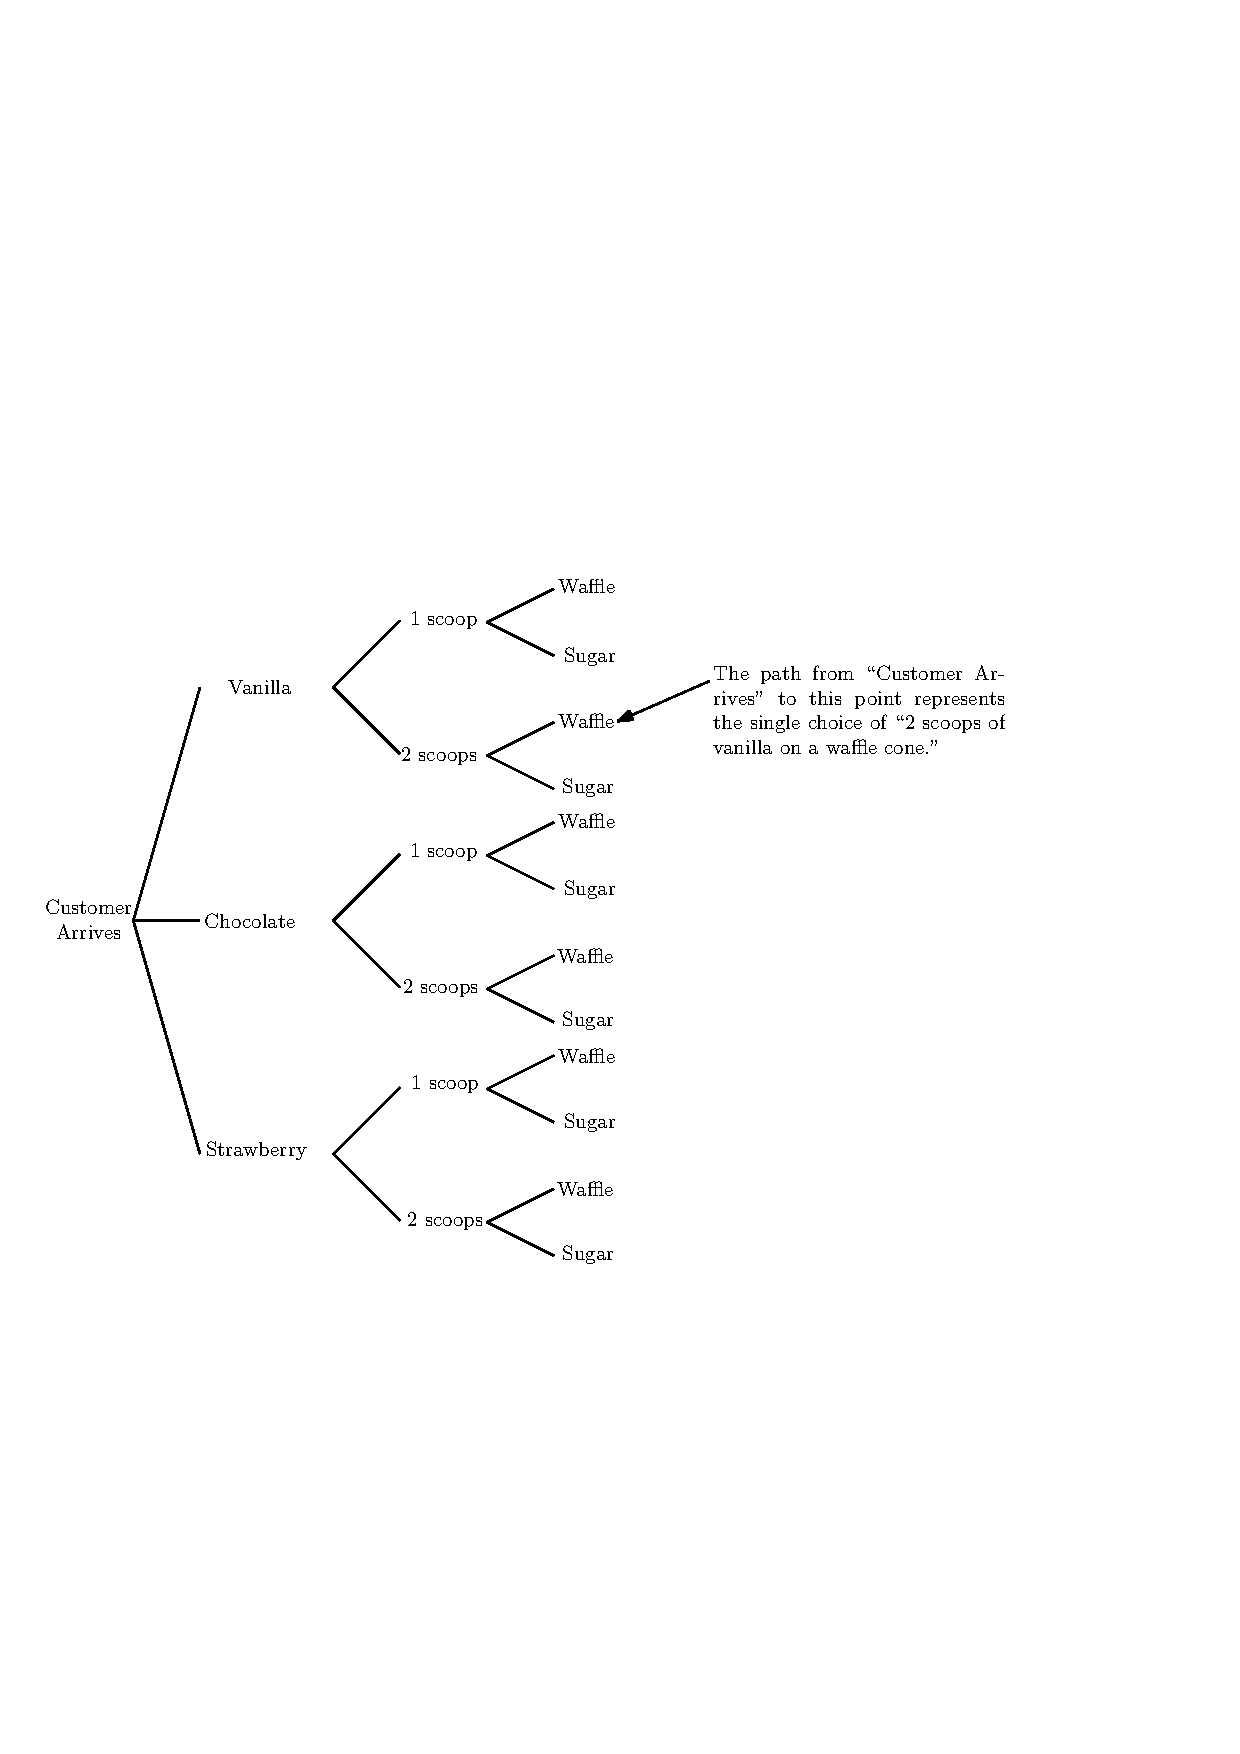
\includegraphics[width=5in]{images/tree2.pdf}
\end{center}
\caption{ Twelve possible orders organized using a tree}\label{systematicPic2}
\end{figure}
}
\wbvfill

\wbvfill

%<*chap1:fundprinc:careful:coneTable>
\item\label{coneTable} Complete the following table as in Question~{\normalfont\ref{sfctable}}.
\begin{center}
\begin{tabular}{|c|c|c||c|}
\hline
Maximum number & Number of & Number of & Number of \\
of scoops & flavors available & types of cones & different orders \\
\hline
$2$ & $5$ & $2$ &  \\
\hline
$3$ & $5$ & $2$ &  \\
\hline
$3$ & $10$ & $2$ &  \\
\hline
$3$ & $f$ & $2$ & \\
\hline
$4$ & $f$ & $2$ &  \\
\hline
$s$ & $f$ & $2$ &  \\
\hline
$s$ & $f$ & $3$ &  \\
\hline
$s$ & $f$ & $4$ &  \\
\hline
$s$ & $f$ & $c$ & \\
\hline
\end{tabular}
\end{center}
%</chap1:fundprinc:careful:coneTable>

\Instr{  Table~{\normalfont\ref{numDiffOrders2}} gives the number of different orders based on the number of scoops, flavors, and cone types available.
\renewcommand{\thetable}{\arabic{chapter}.\arabic{table}(\alph{bluetable})} 
% \setcounter{bluetable}{1}
\addtocounter{table}{-1}
\addtocounter{bluetable}{1}
\begin{table}[htb]
\begin{center}
\begin{tabular}{|c|c|c||c|}
\hline
Maximum number & Number of & Number of & Number of \\
of scoops & flavors available & types of cones & different orders \\
\hline
$2$ & $5$ & $2$ & $2\times 5 \times 2 =20$ \\
\hline
$3$ & $5$ & $2$ & $3\times 5 \times 2 =30$ \\
\hline
$3$ & $10$ & $2$ & $3\times 10 \times 2=60$ \\
\hline
$3$ & $f$ & $2$ & $6\times f$ \\
\hline
$4$ & $f$ & $2$ & $8\times f$ \\
\hline
$s$ & $f$ & $2$ & $s\times f\times 2=2fs$ \\
\hline
$s$ & $f$ & $3$ & $3fs$ \\
\hline
$s$ & $f$ & $4$ & $4fs$ \\
\hline
$s$ & $f$ & $c$ & $s\times f\times c=cfs$\\
\hline
\end{tabular}
\end{center}
\caption{Number of different orders based on the number of scoops, flavors, and cone types available}\label{numDiffOrders2}
\end{table}

You may want to ask the students

\begin{minipage}[H]{5.75in}
\tt \em
\begin{center}
{``Can you choose your cone type before choosing the number of scoops?''}
\end{center}
\end{minipage}

The students should realize that choosing the cone type is independent of choosing the number of scoops. So the order in which you choose your ice cream order does not matter, at this time. 
We will look at situations where choosing the number of scoops and choosing the cone type are \textbf{not} independent events\index{independent event} (that is, the events are dependent\index{dependent}) in Activity~{\normalfont\ref{whatif}}.
}

%<*chap1:fundprinc:careful:truck>
\item Suddenly, a delivery truck arrives with a surplus of ice cream toppings. There are $f$ flavors, up to $s$ scoops, $c$ types of cones, and $t$ toppings available. How many different orders are available at Jack's shack? 
%</chap1:fundprinc:careful:truck>

\Instr{  If the students do not understand this question, ask them what happened to their calculations when they went from two scoops and two flavors to two scoops, two flavors, and two cones. The students should come up with $f\times s \times c \times t$.}



 \wbvfill
\end{enumerate}

\wbnewpage
%<*chap1:fundprinc:whatif:intro>
With $2$ flavors (chocolate and vanilla), up to $5$ scoops, and $2$ cone types (sugar and waffle) available, Jack realizes that a sugar cone cannot handle the weight of the $4^{th}$ or $5^{th}$ scoops. 
%</chap1:fundprinc:whatif:intro>

\begin{enumerate}
%<*chap1:fundprinc:whatif:252>
\setcounter{enumi}{8}
\item\label{252} So he insists that if you order $4$ or $5$ scoops then you must choose the waffle cone. How many different possible ice cream orders are there? Systematically list them all. How do you know that you have them all?
%</chap1:fundprinc:whatif:252>

\Instr{  This would be a good opportunity to have the students use their systematic approach from Question~{\normalfont\ref{systematic}} to exhaust all possible outcomes, or at least show a pattern to recognize the effects. There are $16$ different possible orders.
The students may see the solution as $2 \times 2 \times 1 + 2 \times 3 \times 2=16$ by adding the new possibilities ($2$ flavors, $4$ or $5$ scoops, $1$ cone) to the solution from when there were $2$ flavors, up to $3$ scoops and $2$ cone types are available.

Another way to get this answer is to add the number of different orders that contain a sugar cone only to the number of different orders that contain only the waffle cone. In this way, we would add $2\times 3\times 1=6$ to $2\times 5\times 1=10$ respectively and get $16$ different possible orders.}

\wbvfill

%<*chap1:fundprinc:whatif:unstable>
\item\label{unstable} Even with $3$ scoops, the sugar cone is unstable. Now if you ask for $3$, $4$, or $5$ scoops then you must choose a waffle cone.  What are all the possible ice cream orders now?
%</chap1:fundprinc:whatif:unstable>

\Instr{  Since there are two less possible orders for the sugar cone, we can think of starting with $16$ possible orders with the scoop restriction, there are $2$ less orders. %ordersper. 
So there are a total of $14$ different possible orders.}

\wbvfill
%<*chap1:fundprinc:whatif:previous>
\item How are the answers to Questions~{\normalfont\ref{252}} and {\normalfont\ref{unstable}} different to the entry of the first row in Question~{\normalfont\ref{coneTable}}? How are they the same? 
%</chap1:fundprinc:whatif:previous>

\Instr{  By simply removing the orders which have a sugar cone with $3$, $4$, and $5$ scoops, we have created dependent\index{dependent} events. That is why there are less than $20$ possible orders in the previous two questions compared to the answer in Question~{\normalfont\ref{coneTable}}.}

\wbvfill
%<*chap1:fundprinc:whatif:cake>
\item Jack brings out a $3^{rd}$ cone choice: cake cones. Cake cones can hold up to $3$ scoops, sugar cones can hold up to $2$ scoops and waffle cones can hold up to $5$ scoops. With $2$ flavors available, how many possible orders  are there?
%</chap1:fundprinc:whatif:cake>

\Instr{  If we say there are only $2$ scoops available, then we can treat this problem like in Activity~{\normalfont\ref{careful}}. With up to two scoops available, there are $2\times 3 \times 2$ different orders that can be made. Then there are $2$ additional orders with exactly $3$ scoops in the cake cone. Finally, the waffle cone gives us $6$ additional orders when there are $3$, $4$, and $5$ scoops of ice cream. So we can get $3\times 2\times 2 + 2 + 6 = 20$ orders.

Alternatively: If a cake cone is ordered, there are $2 \times 3=6$ choices; if a sugar cone is ordered, there are $2 \times 2$ choices; and if a waffle cone is ordered, there are $2 \times 5$ choices. These are disjoint events, so we can add them together to get $20$ orders all together.}

\wbvfill
%<*chap1:fundprinc:whatif:tiredRules>
\end{enumerate}

\wbnewpage


%%%%%%%%%  New Subsection  %%%%%%%%%%%%%%%%

\subsection{Activity: Mixing Flavors Is Allowed}\label{whatif}
%</chap1:fundprinc:whatif:tiredRules>

\Instr{  
Goals for this activity:
\begin{packedItem}
\item Developing the specific parameters of a given problem; and
\item using the Fundamental Counting Principle and Tree Diagram counting processes for dependent events.
\end{packedItem}
}

%<*chap1:fundprinc:whatif:tiredRules2>
\indent Customers are tired of all the rules that Jack is enforcing, so they head toward Jill's ice cream parlor. Jill allows customers to have multiple scoops where each scoop can be any flavor no matter whether it is the same or different from the previous one. Jill also places no restriction on the number of scoops allowed in each type of cone.
\begin{enumerate}
\setcounter{enumi}{12}
%</chap1:fundprinc:whatif:tiredRules2>

%<*chap1:fundprinc:whatif:tiredRulesDiff>
\item\label{tiredRulesDiff} With $2$ flavor choices, up to $3$ scoops, and $2$ cone types available, how many different ice cream orders could you possibly have?
%</chap1:fundprinc:whatif:tiredRulesDiff>

\Instr{  Begin by discussing what ``different'' means. The students will get different answers depending on whether they consider chocolate on vanilla as different from vanilla on chocolate. We suggest letting the students begin exploring whichever method of counting they desire. Both methods will be discussed in full detail in Chapter~{\normalfont\ref{perm}} so both scenarios should eventually be explored by the class. Let us say Scenario $1$ is when chocolate on vanilla is different from vanilla on chocolate and Scenario $2$ is when chocolate on vanilla is \textbf{not} different from vanilla on chocolate. 

{\bf Scenario $\bf 1$:} The most natural approach to this problem is to divide the problem into $3$ disjoint\index{disjoint} events (events that cannot occur at the same time): selecting exactly $1$ scoop, exactly $2$ scoops or exactly $3$ scoops.  To get the students thinking along these lines, you may want to ask

\begin{minipage}[H]{5.75in}
\tt \em
\begin{center}
{``Can we divide this problem up into smaller problems so that each student in each group can work on a different part?''}
\end{center}
\end{minipage}

For each of these three smaller problems we can use the Fundamental Counting Principle to find the number of possibilities as follows:
\begin{itemize}
\item {\bf $\bf 1$ scoop:} $2\text{ (types of cone)}\times 2\text{ (flavor choices)} =4$.
\item {\bf $\bf 2$ scoops:} $2\text{ (types of cone)} \times (2\times 2 \text{ (flavor choices for the first, then second scoops)})=8$.
\item {\bf $\bf 3$ scoops:} $2\text{ (types of cone})\times (2\times 2\times 2\text{ (flavor each of $3$ levels)})=16$.
\end{itemize}
Adding these (since they are disjoint events) gives $4+8+16=28$ possible orders as seen in Figure~{\normalfont\ref{iceCreamTree}}.
Notice that this tree shows visually why we need to break the counting into $3$ disjoint events before using the Fundamental Counting Principle\index{Fundamental Counting Principle}.
\renewcommand{\thefigure}{\arabic{chapter}.\arabic{figure}(\alph{bluefigure})} 
% \setcounter{bluefigure}{1}
\addtocounter{figure}{-1}
\addtocounter{bluefigure}{1}
\begin{figure}[htb]
\begin{center}
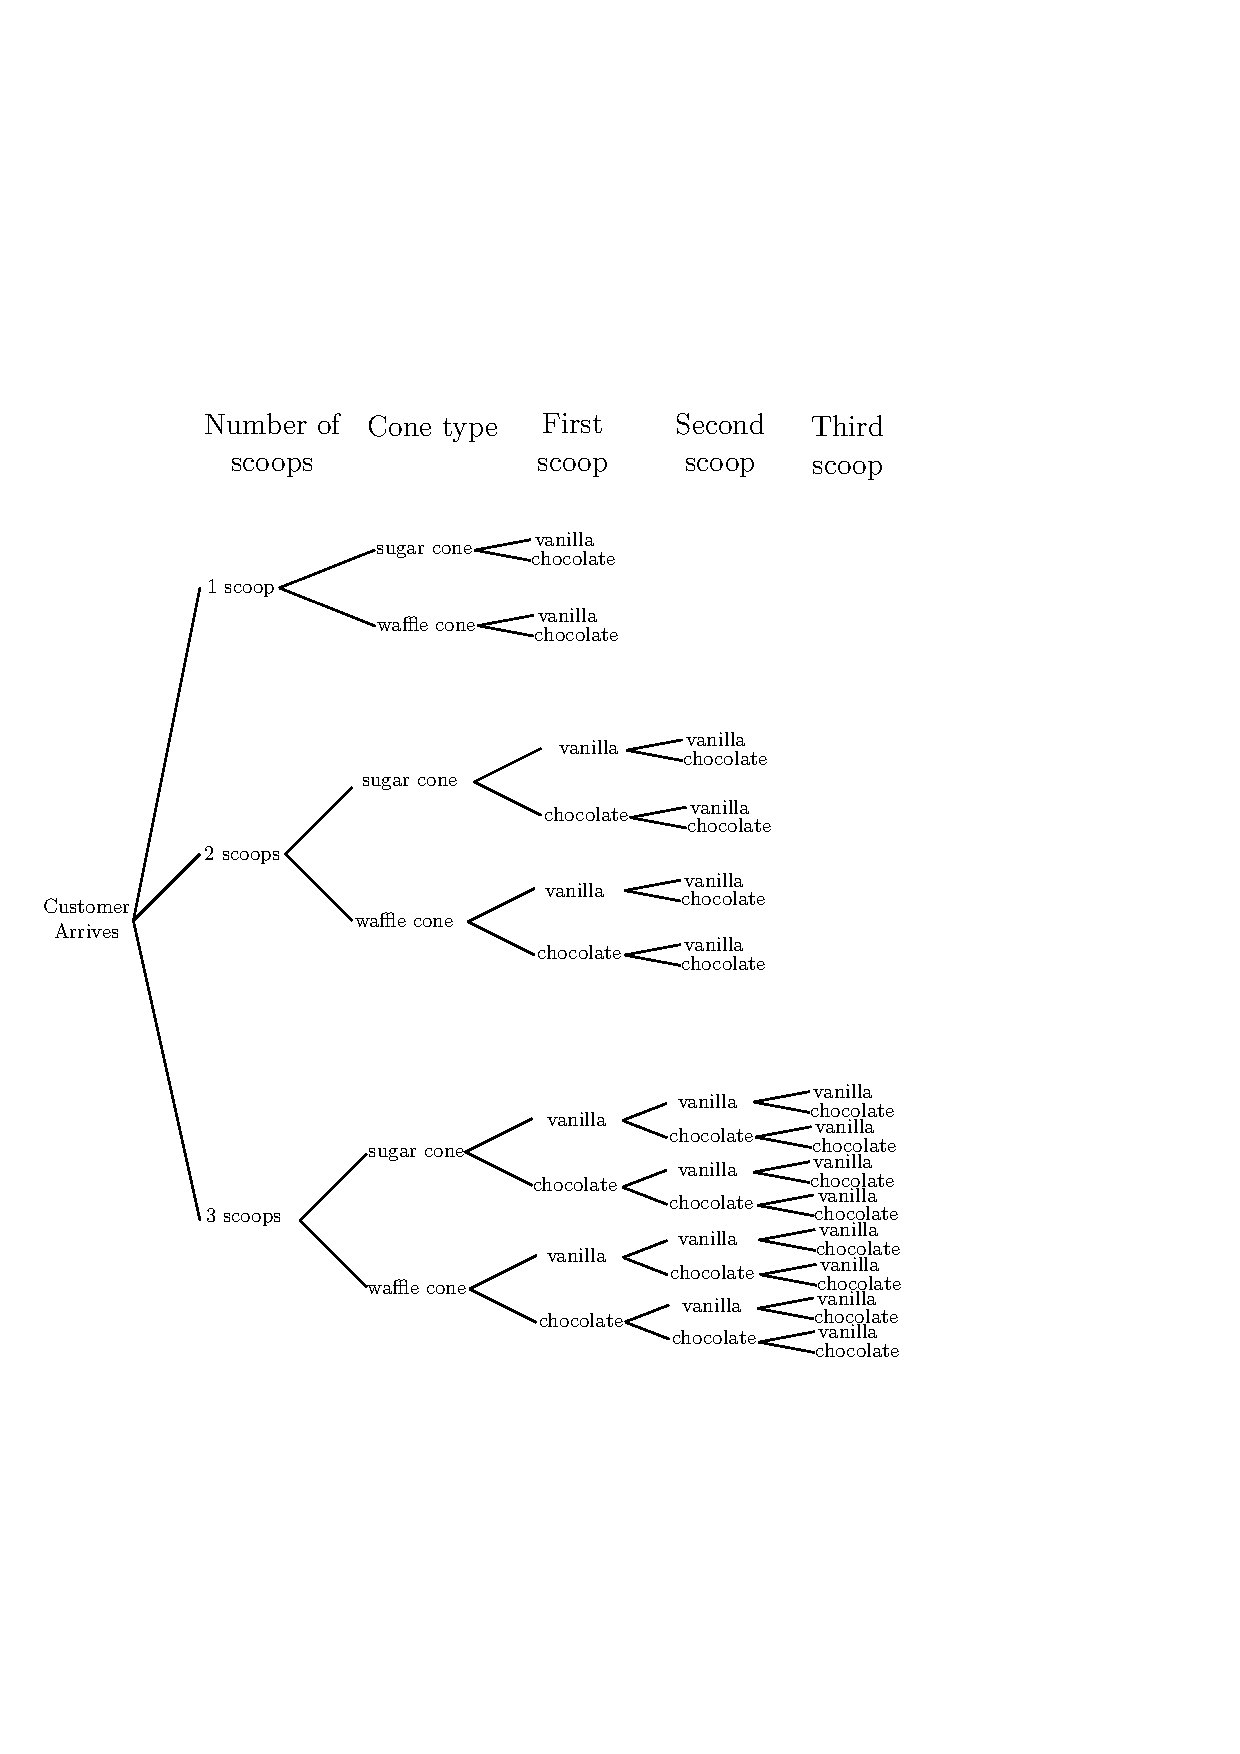
\includegraphics[width=4.5in]{images/iceCreamTree.pdf}
\end{center}
\caption{ $28$ possible orders in Scenario $1$ organized using a tree}\label{iceCreamTree}
\end{figure}

{\bf Scenario $\bf 2$:} The unusual feature in this case is that the choice of flavors is no longer a sequential choice: choosing chocolate then vanilla is now considered the same as choosing vanilla then chocolate, so this must not be counted twice. So if a tree is used to solve the problem, the ``flavor choice'' level would have to be complicated as seen in Figure~{\normalfont\ref{flavorchoice}}.
\renewcommand{\thefigure}{\arabic{chapter}.\arabic{figure}(\alph{bluefigure})} 
% \setcounter{bluefigure}{1}
\addtocounter{figure}{-1}
\addtocounter{bluefigure}{1}
\begin{figure}[htb]
\begin{center}
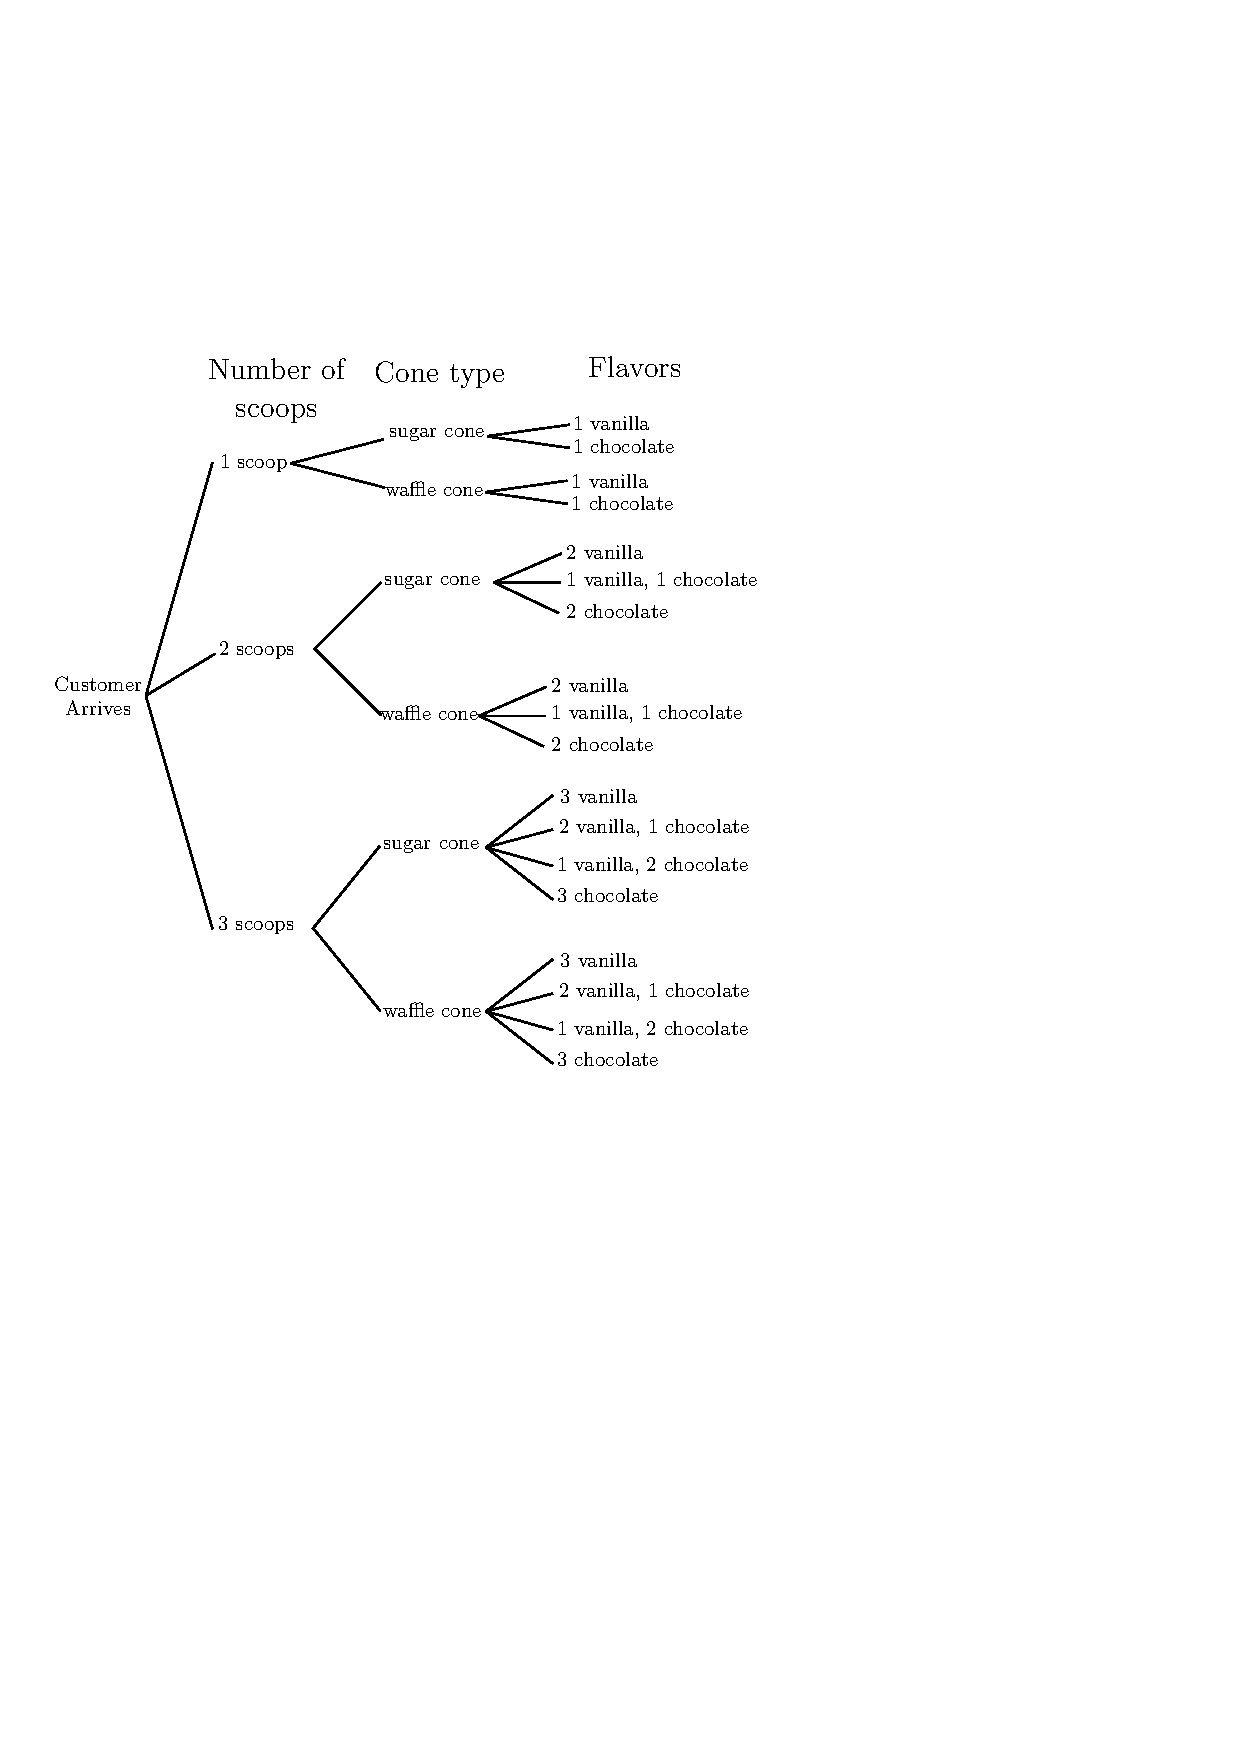
\includegraphics[width=4.5in]{images/flavorChoice.pdf}
\end{center}
\caption{ $18$ possible orders in Scenario $2$ organized using a tree}\label{flavorchoice}
\end{figure}

When only two flavors are available, it is not too difficult to list the``flavor level'' possibilities, but the techniques developed for counting combinations in Chapter~{\normalfont\ref{perm}} do give a better systematic approach to solving this problem in general. 

We can proceed to list out the possible orders as we did in Scenario $1$ by dividing the problem into $3$ disjoint events\index{disjoint event}: selecting exactly $1$ scoop, exactly $2$ scoops, or exactly $3$ scoops. The difficult part to finding the number of orders for each disjoint event is finding the number of ways to choose the flavors. If there is only one scoop, then you could have vanilla or you can have chocolate. But when the number of scoops increases to $2$, you could have $2$ scoops of vanilla, $2$ scoops of chocolate, or you could have $1$ scoop of vanilla and $1$ scoop of chocolate. It may be easier to have the students try to find a pattern to the number of ways to choose the flavors given a particular number of scoops assuming that there are only $2$ flavors to choose from. It turns out that if $s$ is the number of scoops, then there are $s+1$ ways to choose the flavors assuming that there are only $2$ flavors to choose from. So we can use the Fundamental Counting Principle to find the number of possible 
orders as follows:
\begin{itemize}
\item {\bf $\bf 1$ scoop:} $2 \text{ (types of cone)} \times 2\text{ (ways to choose $1$ of the $2$ flavors)}=4$
\item {\bf $\bf 2$ scoops:} $2 \text{ (types of cone)} \times 3\text{ (ways to choose $1$ of the $2$ flavors)}=6$
\item {\bf $\bf 3$ scoops:} $2 \text{ (types of cone)} \times 4\text{ (ways to choose $1$ of the $2$ flavors)}=8$
\end{itemize}
Since these are disjoint events, adding the events gives $4+6+8=18$ possible orders.
}
\wbvfill

%<*chap1:fundprinc:whatif:jill4scoops>
\item\label{jill4scoops} Jill now allows up to $4$ scoops with $2$ flavors and $2$ cone types. How many different orders are there?
%</chap1:fundprinc:whatif:jill4scoops>

\Instr{  {\bf Scenario $\bf 1$:} Proceeding as in Question~{\normalfont\ref{tiredRulesDiff}}:
\begin{itemize}
\item {\bf $\bf 1$ scoop:} $2\times 2=4$
\item {\bf $\bf 2$ scoops:} $2\times (2\times 2)=8$
\item {\bf $\bf 3$ scoops:} $2\times (2\times 2\times 2)=16$
\item {\bf $\bf 4$ scoops:} $2\times (2\times 2\times 2\times 2)=32$
\end{itemize}
So there are $4+8+16+32=60$ possible orders. Notice that we can also use Question~{\normalfont\ref{tiredRulesDiff}} and then add the $32$ new choices when there are exactly $4$ scoops of ice cream in a customers order.

{\bf Scenario $\bf 2$:} Proceeding as in Question~{\normalfont\ref{tiredRulesDiff}}:
\begin{itemize}
\item {\bf $\bf 1$ scoop:} $2\times 2=4$
\item {\bf $\bf 2$ scoops:} $2\times 3=6$
\item {\bf $\bf 3$ scoops:} $2\times 4=8$
\item {\bf $\bf 4$ scoops:} $2\times 5=10$
\end{itemize}
So there are $4+6+8+10=28$ possible orders. Notice that we can also use Question~{\normalfont\ref{tiredRulesDiff}} and then add the $10$ new orders when there are exactly $4$ scoops of ice cream in a customers order.
}

\wbvfill

\wbnewpage

%<*chap1:fundprinc:whatif:jill5scoops>
\item\label{jill5scoops} Jill now allows up to $5$ scoops with $2$ flavors and $2$ cone types. Find how many orders are possible. Can you describe how you would find the number of orders possible with $n$ scoops?
%</chap1:fundprinc:whatif:jill5scoops>

\Instr{  One way to solve this question is to use our solution from Question~{\normalfont\ref{jill4scoops}} and add the number of possible orders there are when an order has exactly $5$ scoops of ice cream. Alternatively, we can just count the number of possible orders as in the previous question.

{\bf Scenario $\bf 1$:} Proceeding as in Question~{\normalfont\ref{tiredRulesDiff}}:
\begin{itemize}
\item {\bf $\bf 1$ scoop:} $2\times 2=4$
\item {\bf $\bf 2$ scoops:} $2\times (2\times 2)=8$
\item {\bf $\bf 3$ scoops:} $2\times (2\times 2\times 2)=16$
\item {\bf $\bf 4$ scoops:} $2\times (2\times 2\times 2\times 2)=32$
\item {\bf $\bf 5$ scoops:} $2\times (2\times 2\times 2\times 2\times 2)=64$
\end{itemize}
So there are $4+8+16+32+64=124$ possible orders. Notice that we can also use Question~{\normalfont\ref{tiredRulesDiff}} and then add the $64$ new orders when there are exactly $5$ scoops of ice cream in a customers order.

{\bf Scenario $\bf 2$:} Proceeding as in Question~{\normalfont\ref{tiredRulesDiff}}:
\begin{itemize}
\item {\bf $\bf 1$ scoop:} $2\times 2=4$
\item {\bf $\bf 2$ scoops:} $2\times 3=6$
\item {\bf $\bf 3$ scoops:} $2\times 4=8$
\item {\bf $\bf 4$ scoops:} $2\times 5=10$
\item {\bf $\bf 5$ scoops:} $2\times 6=12$
\end{itemize}
So there are $4+6+8+10+12=40$ possible orders. Notice that we can also use Question~{\normalfont\ref{tiredRulesDiff}} and then add the $12$ new orders when there are exactly $5$ scoops of ice cream in a customers order.
}

% \vspace{.5in}
\wbvfill
%<*chap1:fundprinc:whatif:jill432>
\item\label{jill432} Suppose that Jill considers an order of chocolate on vanilla to be different from an order with vanilla on chocolate. Find the number of possible orders you can make when Jill allows up to $2$ cone types, up to $4$ scoops, and $3$ different flavors available.
%</chap1:fundprinc:whatif:jill432>

\Instr{  Notice that this question is only asking about Scenario $1$. So any class that decided to focus solely on Scenario $2$ should omit Questions~{\normalfont\ref{jill432}} and {\normalfont\ref{whatif:describe}}. Question~{\normalfont\ref{whatif:describe}} addresses the general solution to the counting problem under Scenario $1$. The solution to this counting problem under Scenario $2$ becomes much more difficult with our current counting methods when more than $2$ flavors are allowed. In Activity~{\normalfont\ref{whichIceCreamIsDifferent}}, having developed new counting methods, the general solution to this counting problem under Scenario $2$ is investigated.

{\bf Scenario $\bf 1$:} The calculations are remarkably similar to those performed in Question~{\normalfont\ref{tiredRulesDiff}}. The only difference is that at each ``flavor level'' we now have $3$ choices instead of $2$.
\begin{itemize}
\item {\bf ${\bf 1}$ scoop:} $2\times 3=6$
\item {\bf ${\bf 2}$ scoops:} $2\times (3\times 3)=18$
\item {\bf ${\bf 3}$ scoops:} $2\times (3\times 3\times 3)=54$
\item {\bf ${\bf 4}$ scoops:} $2\times (3\times 3\times 3\times 3)=162$
\end{itemize}
So there are $6+18+54+162=240$ possible orders. }

\wbvfill

%<*chap1:fundprinc:whatif:describe>
\item\label{whatif:describe} Suppose that Jill considers an order of chocolate on vanilla to be different from an order with vanilla on chocolate. Can you describe a method for finding the number of possible orders with up to $s$ scoops, $f$ flavors, and $2$ cone types available?
%</chap1:fundprinc:whatif:describe>

\Instr{  By rigorously going through Questions~{\normalfont\ref{jill4scoops}}, {\normalfont\ref{jill5scoops}}, and {\normalfont\ref{jill432}}, it can be seen that the number of flavors follows a specific pattern. Remember that we are only working with Scenario $1$ according to the question statement.

{\bf Scenario $\bf 1$:} If there are exactly $x$ scoops of ice cream, then there are $x$ ``flavor levels'' to the tree. So there are $f$ choices at each level of the tree. Since there are $2$ cone choices and by the Fundamental Counting Principle there are 
$$2\times \underbrace{f\times f \times \cdots \times f}_{x \text{ times}}=2f^x$$
possible orders with exactly $x$ scoops of ice cream. So by adding the number of possible orders with exactly $x$ scoops for all $1\leq x \leq s$, we get $2f+2f^2+2f^3+2f^4+\cdots+2f^{s+1}$ possible orders of ice cream.
}

\wbvfill
\wbnewpage
%<*chap1:fundprinc:whatif:jackandjill>
\end{enumerate}
% \item\label{jackandjill} 

\indent Jack and Jill join together to set up the ice cream emporium on top of a near by hill. Each sees that some of the other's rules have merit. They decide that customers are now allowed to have a different flavor for each scoop, sugar cones can hold up to $2$ scoops, cake cones can hold up to $3$ scoops, and waffle cones can hold up to $5$ scoops. They are willing to let you decide whether or not chocolate on vanilla should be considered different from vanilla on chocolate. (Keen young minds may want to consider both options!)
\begin{enumerate}
\setcounter{enumi}{17}
%</chap1:fundprinc:whatif:jackandjill>
% \begin{enumerate}
%<*chap1:fundprinc:whatif:252jackjill>
\item\label{252jackjill} How many possible orders can be made with $2$ flavors, up to $5$ scoops, and only waffle and sugar cones allowed. 
%</chap1:fundprinc:whatif:252jackjill>

\Instr{  We can use our answer from Question~{\normalfont\ref{jill5scoops}} to help us solve this question. All we need to do is remove the orders that cannot be bought. For example, we cannot order a sugar cone with $5$ scoops. For Scenario $1$, there are $124-6-30-14-6=68$ possible orders. For Scenario $2$, there are $40-6-4-3-2=25$ possible orders.

Another possible way to attack this problem is to go through the full process of finding the number of orders possible for each number of scoops as in Question~{\normalfont\ref{tiredRulesDiff}} and {\normalfont\ref{jill5scoops}}. So we split this problem up into $5$ disjoint events\index{disjoint event} depending on the number of scoops. Since we only have waffle cones and sugar cones, the solutions to Scenario $1$ and Scenario $2$ with $1$ and $2$ scoops will be identical to those we calculated in Question~{\normalfont\ref{jill5scoops}} since having $1$ or $2$ scoops does not affect which cones we can choose. For $3$, $4$ and $5$ scoops, we must be careful to note that we are not allowed to use the sugar cone anymore. 

{\bf Scenario $\bf 1$:} As we said earlier, we know the number of possible orders when the number of scoops is $1$ or $2$ from Question~{\normalfont\ref{jill5scoops}}. For $3$, $4$, and $5$ scoops, it is important to realize the number of flavor choices for the $s$ levels of ice cream does not change even though we can only use $1$ cone. So we can use the Fundamental Counting Principle\index{Fundamental Counting Principle} to find the number of possible orders as follows:
\begin{itemize}
\item {\bf $\bf 1$ scoop:} $2 \text{ (types of cone)} \times 2 \text{ (flavor choices)} =4$ 
\item {\bf $\bf 2$ scoops:} $2 \text{ (types of cone)} \times (2\times 2 \text{ (flavor choices)}) =8$ 
\item {\bf $\bf 3$ scoops:} $1 \text{ (type of cone)} \times (2\times 2 \times 2\text{ (flavor choices)}) =8$ 
\item {\bf $\bf 4$ scoops:} $1 \text{ (type of cone)} \times (2\times 2 \times 2 \times 2 \text{ (flavor choices)}) =16$ 
\item {\bf $\bf 5$ scoops:} $1 \text{ (type of cone)} \times (2\times 2 \times 2 \times 2 \times 2 \text{ (flavor choices)}) =32$ 
\end{itemize}
So there are $4+8+8+16+32=68$ possible orders of ice cream.


{\bf Scenario $\bf 2$:} Again, we know the number of possible orders when the number of scoops is $1$ or $2$ from Question~{\normalfont\ref{jill5scoops}}. As in Scenario $1$, for $3$, $4$, and $5$, it is important for the students to realize the number ways to choose the flavors of ice cream does not change even though we can only use $1$ cone. So we can use the Fundamental Counting Principle\index{Fundamental Counting Principle} to find the number of possible orders as follows:
\begin{itemize}
\item {\bf $\bf 1$ scoop:} $2 \text{ (types of cone)} \times 2 \text{ (ways to choose $1$ of the $2$ flavors)} = 4$
\item {\bf $\bf 2$ scoops:} $2 \text{ (types of cone)} \times 3 \text{ (ways to choose $1$ of the $2$ flavors)} = 6$ 
\item {\bf $\bf 3$ scoops:} $1 \text{ (type of cone)} \times 4 \text{ (ways to choose $1$ of the $2$ flavors)} = 4$
\item {\bf $\bf 4$ scoops:} $1 \text{ (type of cone)} \times 5 \text{ (ways to choose $1$ of the $2$ flavors)} = 5$
\item {\bf $\bf 5$ scoops:} $1 \text{ (type of cone)} \times 6 \text{ (ways to choose $1$ of the $2$ flavors)} = 6$
\end{itemize}
So there are $4+6+4+5+6=25$ possible orders of ice cream.
}

% \vspace{.5in}
\wbvfill

%<*chap1:fundprinc:whatif:253jackjill>
\item Suppose there are $2$ flavors, up to $5$ scoops, and we can choose a waffle cone, sugar cone, or cake cone for our cone type. How many possible orders are there?
%</chap1:fundprinc:whatif:253jackjill>

\Instr{  We can follow a similar procedure to the one outlined in Question~{\normalfont\ref{252jackjill}}. Again we split this problem into $5$ disjoint events\index{disjoint event} based on the number of scoops chosen.

{\bf Scenario $\bf 1$:} As in Question~{\normalfont\ref{252jackjill}}, the number of flavor choices for the $s$ levels of ice cream does not change even if the number of cone types changes. This is because these are independent events\index{independent event}. So we can use the Fundamental Counting Principle\index{Fundamental Counting Principle} to find the number of possible orders as follows:
\begin{itemize}
\item {\bf $\bf 1$ scoop:} $3 \text{ (types of cones)} \times 2 \text{ (flavor choices)} =6$
\item {\bf $\bf 2$ scoops:} $3 \text{ (types of cones)} \times (2\times 2 \text{ (flavor choices)}) =12$ 
\item {\bf $\bf 3$ scoops:} $2 \text{ (types of cones)} \times (2\times 2\times 2 \text{ (flavor choices)}) =16$
\item {\bf $\bf 4$ scoops:} $1 \text{ (type of cones)} \times (2\times 2 \times 2 \times 2 \text{ (flavor choices)}) =16$
\item {\bf $\bf 5$ scoops:} $1 \text{ (type of cones)} \times (2\times 2 \times 2 \times 2 \times 2 \text{ (flavor choices)}) =32$
\end{itemize}
Since each of these events are disjoint, the number of possible orders is $6+12+16+16+32=82$.

{\bf Scenario $\bf 2$:} As in Question~{\normalfont\ref{252jackjill}}, it is important for the students to realize the number ways to choose the flavors of ice cream does not change even if the number of cone types changes. So we can use the Fundamental Counting Principle\index{Fundamental Counting Principle} to find the number of possible orders as follows:
\begin{itemize}
\item {\bf $\bf 1$ scoop:} $3 \text{ (types of cone)} \times 2 \text{ (ways to choose $1$ of the $2$ flavors)} = 6$
\item {\bf $\bf 2$ scoops:} $3 \text{ (types of cone)} \times 3 \text{ (ways to choose $1$ of the $2$ flavors)} = 9$
\item {\bf $\bf 3$ scoops:} $2 \text{ (types of cone)} \times 4 \text{ (ways to choose $1$ of the $2$ flavors)} = 8$
\item {\bf $\bf 4$ scoops:} $1 \text{ (type of cone)} \times 5 \text{ (ways to choose $1$ of the $2$ flavors)} = 5$
\item {\bf $\bf 5$ scoops:} $1 \text{ (type of cone)} \times 6 \text{ (ways to choose $1$ of the $2$ flavors)} = 6$
\end{itemize}
Since each of these events are disjoint\index{disjoint event}, the number of possible orders of ice cream is $6+9+8+5+6=34$.
}

\wbvfill

%<*chap1:fundprinc:whatif:353jackjill>
\item Jack and Jill go up the hill to their ice cream emporium and find a delivery of a third flavor: strawberry ice cream. With the $3$ flavors, up to $5$ scoops, and $3$ cone types available, how many possible orders are there?
%</chap1:fundprinc:whatif:353jackjill>

\Instr{  As said in Question~{\normalfont\ref{tiredRulesDiff}}, things will get more difficult now that the number of flavors has increased to $3$. Fortunately, once we find the number of flavor choices for a particular number of scoops of ice cream, the number of flavor choices does not change even if the number of cone types available does change.
We begin by dividing this problem into five disjoint cases based on the number of scoops of ice cream. 

{\bf Scenario $\bf 1$:} If there are $3$ possible flavors, then each scoop level has $3$ possible choices for flavor. So if there are $s$ scoops of ice cream available, the Fundamental Counting Principle tells us there are $3\times 3 \times 3\times \cdots  \times 3=3^s$ possible flavor choices. Since the number of cone types is independent\index{independent event} of the number of flavor choices, we can use the Fundamental Counting Principle\index{Fundamental Counting Principle} to find the number of possible orders of ice cream as follows:
\begin{itemize}
\item {\bf $\bf 1$ scoop:} $3 \text{ (types of cones)} \times 3 \text{ (flavor choices)} =9$
\item {\bf $\bf 2$ scoops:} $3 \text{ (types of cones)} \times (3\times 3 \text{ (flavor choices)}) =27$ 
\item {\bf $\bf 3$ scoops:} $2 \text{ (types of cones)} \times (3\times 3\times 3 \text{ (flavor choices)}) =54$
\item {\bf $\bf 4$ scoops:} $1 \text{ (type of cones)} \times (3\times 3 \times 3 \times 3 \text{ (flavor choices)}) =81$
\item {\bf $\bf 5$ scoops:} $1 \text{ (type of cones)} \times (3\times 3 \times 3 \times 3 \times 3 \text{ (flavor choices)}) =243$
\end{itemize}
Since each of these events are disjoint, the number of possible orders is $9+27+54+81+243=414$.

{\bf Scenario $\bf 2$:} As in Scenario $1$, all we need to do is find the number of possible flavor choices for each particular number of scoops. But this will be difficult since we do not have the proper tools to count the number of ways to arrange $3$ flavors yet. The only option we have available to us right now is to count the numbers out exclusively for each number of scoops. For $1$ scoop it is easy to see that we only have $3$ possible flavor choices: $1$ scoop of vanilla, $1$ scoop of chocolate, or $1$ scoop of strawberry. By writing out each of the possible flavor choices for each number of scoops you should find that there are $6$, $10$, $15$, and $21$ flavor choices for $2$, $3$, $4$, and $5$ scoops of ice cream respectively. There is a pattern that the students could discover to make their lives easier. By using the previous number of scoops, you can determine how many flavor choices will be available for the current number of scoops. Since the number of cone types is independent\index{independent event} of the number of flavor choices, we can use 
the Fundamental Counting Principle\index{Fundamental Counting Principle} to find the number of possible orders of ice cream as follows:
\begin{itemize}
\item {\bf $\bf 1$ scoop:} $3 \text{ (types of cone)} \times 3 \text{ (ways to choose $1$ of the $3$ flavors)} = 9$
\item {\bf $\bf 2$ scoops:} $3 \text{ (types of cone)} \times 6 \text{ (ways to choose $1$ of the $3$ flavors)} = 18$
\item {\bf $\bf 3$ scoops:} $2 \text{ (types of cone)} \times 10 \text{ (ways to choose $1$ of the $3$ flavors)} = 20$
\item {\bf $\bf 4$ scoops:} $1 \text{ (type of cone)} \times 15 \text{ (ways to choose $1$ of the $3$ flavors)} = 15$
\item {\bf $\bf 5$ scoops:} $1 \text{ (type of cone)} \times 21 \text{ (ways to choose $1$ of the $3$ flavors)} = 21$
\end{itemize}
Since each of these events are disjoint\index{disjoint event}, the number of possible orders of ice cream is $9+18+20+15+21=83$.
}
\wbvfill

% \end{enumerate} 
\end{enumerate}
\wbnewpage


%%%%%%%%%  New Subsection  %%%%%%%%%%%%%%%%

\subsection{Activity: Which ice cream is different?}\label{whichIceCreamIsDifferent}

\indent Jill allows customers to have multiple scoops where each scoop can be the same or different from the other scoops but she considers an order with chocolate on top of vanilla to be the same as an order with vanilla on chocolate.
%</chap1:extension:whichIceCream:intro>

\Instr{  Answering these questions in general with the techniques we have is not easy, but will be easy by the end of Chapter~{\normalfont\ref{perm}}. It is good to approach these questions in a systematic way so as not to miss any combinations.}

%<*chap1:extension:whichIceCream:intro2>
\begin{enumerate}
%\setcounter{enumi}{14}
\setcounter{enumi}{20}
\item\label{123comboIceCream} If Jill has only $1$ cone type, up to two scoops, and $3$ flavors are available to her customers, how many possible orders are there?
%</chap1:extension:whichIceCream:intro2>

\Instr{  Notice that if we consider chocolate on vanilla to be the same order as vanilla on chocolate, then we are in Scenario $2$ from Question~{\normalfont\ref{tiredRulesDiff}} of Activity~{\normalfont\ref{whatif}}. This question becomes much more difficult if there are $3$ flavors instead of $2$. As in Question~{\normalfont\ref{tiredRulesDiff}} of Activity~{\normalfont\ref{whatif}} we can still divide this problem into $2$ cases: selecting exactly $1$ scoop or exactly $2$ scoops. By listing all the different ways to get $2$ scoops of ice cream with $3$ different flavors, it is quickly seen that there are $6$ different combinations: vanilla and vanilla, chocolate and chocolate, strawberry and strawberry, vanilla and chocolate, vanilla and strawberry, and finally chocolate and strawberry.
So there are $3$ possible flavor choice with $1$ scoop and $6$  flavor choices with $2$ scoops and thus $6+3=9$ possible orders since we only have one cone type available.
Figure~{\normalfont\ref{iceCreamCombos2Scoops}} gives a visual representation of the number of possible orders organized as we described above.
\renewcommand{\thefigure}{\arabic{chapter}.\arabic{figure}(\alph{bluefigure})} 
%  \setcounter{bluefigure}{1}
\addtocounter{figure}{-1}
\addtocounter{bluefigure}{1}
\begin{figure}[htb]
\begin{center}
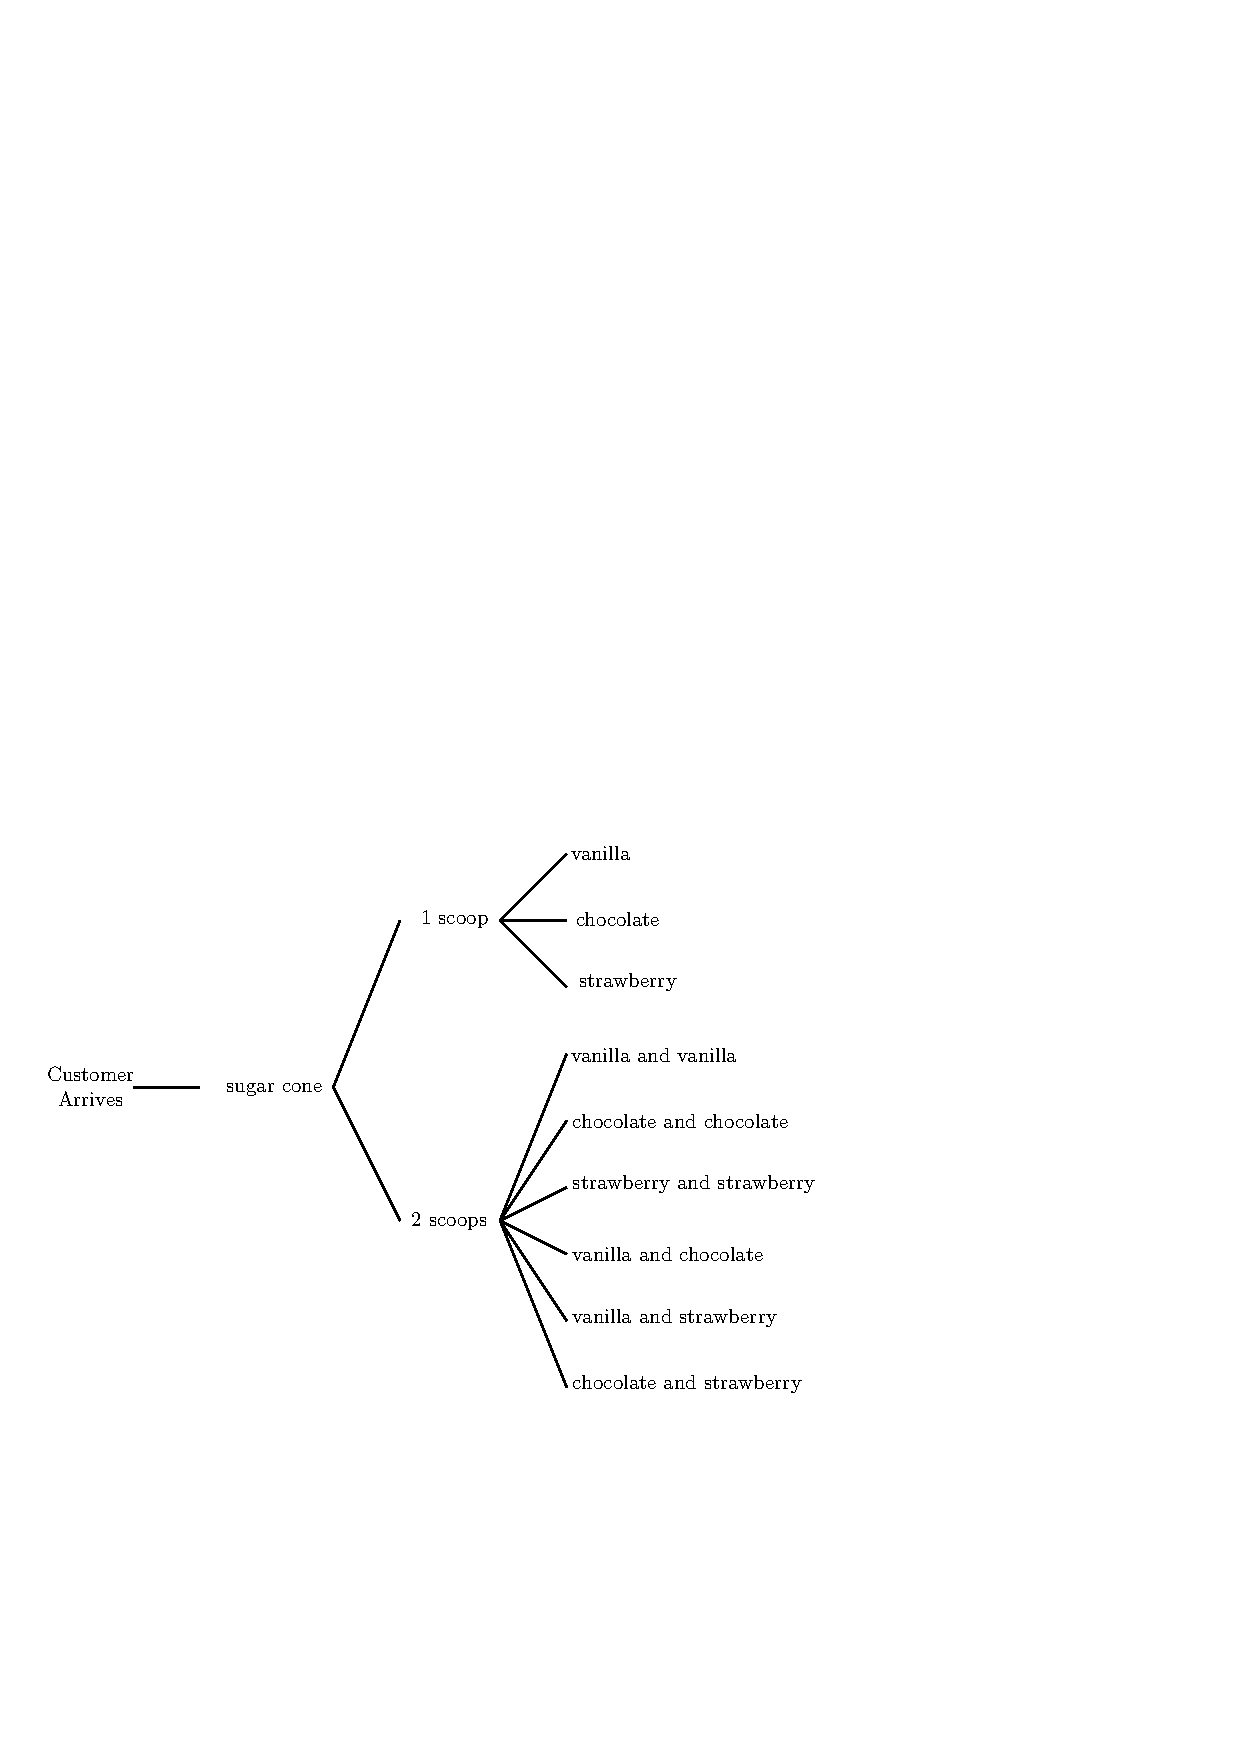
\includegraphics[width=5in]{images/iceCreamCombos2Scoops.pdf}
\end{center}
\caption{ $9$ possible orders in Scenario $2$ organized using a tree}\label{iceCreamCombos2Scoops}
\end{figure}
}

\wbvfill

%<*chap1:extension:whichIceCream:133comboIceCream>
\item\label{133comboIceCream} If Jill has only $1$ cone type, up to $3$ scoops, and $3$ flavors are available to her customers, how many possible order are there?
%</chap1:extension:whichIceCream:133comboIceCream>

\Instr{  For this problem we can use Question~{\normalfont\ref{123comboIceCream}} and add the number of ways to order $3$ scoops, so we can use the selections at the ``flavor level'' of the tree in Table~{\normalfont\ref{flavorLevelTable}}, where $v=$vanilla, $c=$chocolate, and $s=$strawberry.
\renewcommand{\thetable}{\arabic{chapter}.\arabic{table}(\alph{bluetable})} 
%  \setcounter{bluetable}{1}
\addtocounter{table}{-1}
\addtocounter{bluetable}{1}
\begin{table}[htb]
\begin{center}
\begin{tabular}{ccccc}
\multicolumn{5}{c}{Scoop flavors} \\
\cline{2-4}
& \multicolumn{1}{|c}{$v$} & $v$ & \multicolumn{1}{c|}{$v$} & \\
\cline{2-4}
& \multicolumn{1}{|c}{$c$} & $c$ & \multicolumn{1}{c|}{$c$} \\
\cline{2-4}
& \multicolumn{1}{|c}{$s$} & $s$ & \multicolumn{1}{c|}{$s$} \\
\cline{2-4}
& \multicolumn{1}{|c}{$v$} & $c$ & \multicolumn{1}{c|}{$c$} \\
\cline{2-4}
& \multicolumn{1}{|c}{$v$} & $s$ & \multicolumn{1}{c|}{$s$} \\
\cline{2-4}
& \multicolumn{1}{|c}{$c$} & $v$ & \multicolumn{1}{c|}{$v$} \\
\cline{2-4}
& \multicolumn{1}{|c}{$c$} & $s$ & \multicolumn{1}{c|}{$s$} \\
\cline{2-4}
& \multicolumn{1}{|c}{$s$} & $c$ & \multicolumn{1}{c|}{$c$} \\
\cline{2-4}
& \multicolumn{1}{|c}{$s$} & $v$ & \multicolumn{1}{c|}{$v$} \\
\cline{2-4}
& \multicolumn{1}{|c}{$s$} & $c$ & \multicolumn{1}{c|}{$v$} \\
\cline{2-4}
\end{tabular}
\end{center}
\caption{List of possible flavors with $3$ scoops of ice cream}\label{flavorLevelTable}
\end{table}
So there are $10$ new selections at the ``flavor level'' and thus $9+10=19$ possible orders.
Finding the number of ways to choose $r$ object types from a set of size $s$ where object types can be repeated is addressed in Activity~{\normalfont\ref{stickyNotes}}.
}
%</chap1:icecream>
\wbvfill

%<*chap1:icecreamextension>
%<*chap1:extension:whichIceCream:end>
\end{enumerate}
%</chap1:extension:whichIceCream:end>

%</discreteCounting.intro4ChanceOfSomethingTasty>

%<*discreteCounting.intro5PredictingIceCream>

\wbnewpage



%%%%%%%%%  New Subsection  %%%%%%%%%%%%%%%%

\subsection{Exit Activity: Area Codes}

Originally area codes were made up of three numbers ($0$ through $9$) where the middle digit was either $0$ or $1$ and the first digit was non-zero. 
\begin{enumerate}
\item\label{areaCodesA} In this way, how many different area codes were possible?
%</chap1:exercises:areaCodesA>

\Instr{  
Choosing a number for the first digit does not affect the number of choices we have for subsequent digits. The same is true for each pair of digits. So we may use the Fundamental Counting Principle. The first digit cannot be $0$ so there are $9$ possibilities to choose from. The second digit can only be $0$ or $1$ which gives $2$ possibilities for this digit. The last digit has no restrictions, so there are $10$ possibilities. Thus, the number of ways to form an area code at this time is $9\times 2 \times 10=180$.
}

\wbvfill

%<*chap1:exercises:areaCodesB>
\item To avoid emergency contact numbers such as $911$ and $411$ no area code is allowed to end with consecutive $1$'s. How many different area codes were there if all area codes that end in $11$ were forbidden?
%</chap1:exercises:areaCodesB>

\Instr{ 
By using our solution from Question~{\normalfont\ref{areaCodesA}}, all we need to do is find the number of forbidden numbers and subtract it from $180$ possible area codes. A forbidden configuration contains two consecutive $1$ at the end of the area code, so they would be of the form $?11$. Thus there are ten area codes of forbidden configurations of the form $?11$. So there are $180-9=171$ area codes of the specified form.
}
\wbvfill

%<*chap1:exercises:endSteveDice>
\end{enumerate}

\wbnewpage


%<*chap1:extension:predictingIceCream:title>
\subsection{Extension Activity: A Chance of Something Tasty}\label{predictingIceCream}
%</chap1:extension:predictingIceCream:title>

%<*chap1:extension:predictingIceCream:intro>
In discrete settings in which all outcomes are equally likely to occur, probability calculations rely on being able to count well. The probability of a certain event $E$ occurring is simply the number of outcomes that satisfy the event $E$ divided by the total number of possible outcomes. So our efforts to consolidate counting techniques will stand us in good stead as the following questions are addressed.

Jill's ice cream parlor allows customers to have multiple scoops where each scoop can be the same or different to the previous flavor choices. Jill also places no restriction on the number of scoops allowed in each type of cone. 

Any order can have: 
\begin{itemize}
\setcounter{enumi}{26}
\item[$(i)$] up to $3$ scoops, with $2$ flavor choices (vanilla and chocolate), and $2$ choices of cone type (waffle and sugar). 
\end{itemize}
Also, it is important to know that:
\begin{itemize}
\item[$(ii)$] at this time, Jill considers that having chosen the cone type, putting vanilla on top of chocolate in the cone is the \textbf{same} as putting chocolate on top of vanilla (so it is just the number of scoops of each flavor that matters). 
\end{itemize}

Late one night, Jill wonders what the probability is for a particular type of order to be requested, assuming that:
\begin{itemize}
\item[$(iii)$] each order of ice cream has equal probability of occurring. 
\end{itemize}
%</chap1:extension:predictingIceCream:intro>

%<*chap1:extension:predictingIceCream:prob2vanSug>
\begin{enumerate}
\item\label{prob2vanSug} What is the probability that a customer orders exactly $2$ scoops, both being vanilla, on a sugar cone? 
%</chap1:extension:predictingIceCream:prob2vanSug>

\Instr{  
To find the probability of a particular order of ice cream we must first count the number of different possible orders. The number of possible orders was already found in Question~{\normalfont\ref{tiredRulesDiff}} of Activity~{\normalfont\ref{whatif}}. There are $18$ different possible orders. Next, we must find the number of orders that include exactly $2$ scoops of vanilla on a sugar cone. The description of ordering exactly $2$ scoops of vanilla on a sugar cone is commonly called an event\index{event}. We need to find out the number of times this event can occur. There is only $1$ order that fits this description. Since each order has an equal probability of occurring, the probability of ordering exactly $2$ scoops of vanilla on a sugar cone is $1/18 \approx 0.0556$. 
}

%<*chap1:extension:predictingIceCream:prob2van>
\item\label{prob2van} What is the probability that a customer orders precisely $2$ scoops, both being vanilla, on any cone?
%</chap1:extension:predictingIceCream:prob2van>

\Instr{ 
As said in Question~{\normalfont\ref{prob2vanSug}}, we must know the number of possible ice cream orders. There are $18$ different possible orders. Now we must find the number of orders that contain exactly $2$ scoops of vanilla. There are two such orders: $2$ scoops of vanilla on a sugar cone and $2$ scoops of vanilla on a waffle cone. So the probability of ordering exactly $2$ scoops of vanilla is $2/18=1/9\approx 0.1111$.
}

%<*chap1:extension:predictingIceCream:prob>=2van>
\item What is the probability that the customers' order includes $2$ scoops of vanilla ice cream on a sugar cone?
%</chap1:extension:predictingIceCream:prob>=2van>

\Instr{ 
Since the order only has to contain $2$ scoops of vanilla, it is possible that the third scoop is chocolate. So we can separate this problem into two disjoint events: exactly $2$ scoops of ice cream and exactly $3$ scoops of ice cream. In Question~{\normalfont\ref{prob2vanSug}}, we already found that there is $1$ order that contains exactly $2$ scoops of ice cream. We now turn to counting the number of orders that contain exactly $3$ scoops of ice cream. Since the order in which the ice cream is placed on the cone does not matter, there are two ways to have three scoops of ice cream: $3$ scoops of vanilla or $2$ scoops of vanilla and $1$ scoop of chocolate. With $1$ choice of cone, it is clear there are $2\times 1=2$ orders that contain exactly $3$ scoops of ice cream. So there are $1+2=3$ orders that include $2$ scoops of vanilla ice cream on a sugar cone and thus the probability of ordering $2$ scoops of vanilla on a sugar cone is $3/18=1/6=0.1666$.
}

%<*chap1:extension:predictingIceCream:prob2>
\item\label{prob2} What is the probability that a customer orders exactly $2$ scoops of any flavors of ice cream on any cone type?
%</chap1:extension:predictingIceCream:prob2>

\Instr{ 
There are $18$ possible orders as said in Question~{\normalfont\ref{prob2vanSug}} Now we must find the number of orders that contain $2$ scoops of ice cream. There are six such orders: $2$ scoops of vanilla on a sugar cone, $2$ scoops of vanilla on a waffle cone, $1$ scoop of vanilla and $1$ scoop of chocolate on a waffle cone, $1$ scoop of vanilla and $1$ scoop of chocolate on a sugar cone, $2$ scoops of chocolate on a sugar cone, and $2$ scoops of chocolate on a waffle cone. So the probability of ordering $2$ scoops of ice cream is $6/18=1/3\approx 0.6667$. 
}

%<*chap1:extension:predictingIceCream:prob<=2>
\item What is the probability that a customer orders at most $2$ scoops of any flavors of ice cream on any cone type?
%</chap1:extension:predictingIceCream:prob<=2>

\Instr{ 
There are $18$ possible orders as said in Question~{\normalfont\ref{prob2vanSug}}. Now we must find the number of orders that contain at most $2$ scoops of ice cream. By Question~{\normalfont\ref{prob2}}, we know there are $6$ orders that have $2$ scoops. There are $4$ orders that have $1$ scoop. So the probability of ordering at most $2$ scoops of ice cream is $(6+4)/18=5/9 \approx 0.5556$. 
}

%<*chap1:extension:predictingIceCream:endDiff>
\end{enumerate}
%</chap1:extension:predictingIceCream:endDiff>

%</discreteCounting.intro5PredictingIceCream>

%<*discreteCounting.intro6ColdCalculations>



\wbnewpage

%%%%%%%%%%%%%%%%%%%%%%%%%%%%%%%%%%%%%%%%
%%%%%%%%%  New Section  %%%%%%%%%%%%%%%%
%%%%%%%%%%%%%%%%%%%%%%%%%%%%%%%%%%%%%%%%


%<*perm:raceselection:intro:title>
\section{Activity: Mario's Charity Raffle}\label{raceselection}
%</perm:raceselection:intro:title>

\Instr{  
Goals for this activity:
\begin{packedItem}
\item Using Tree Diagrams to determine the number of permutations; and
\item developing an abstract permutation formula.
\end{packedItem}
}


%%%%%%%%%  New Subsection  %%%%%%%%%%%%%%%%


\subsection{Entrance Activity}
%<*perm:raceselection:intro>
A local charity fund raiser has decided to run a raffle. Five balls are placed in an opaque box (the five balls are marked $1$, $2$, $3$, $4$, and $5$ respectively). When the raffle begins, one or more balls will be chosen and announced. Currently the raffle consists of choosing one ball and then choosing a second ball \emph{without} replacing the first ball in the box. Each participant donates to the charity, then writes down which ball they think will be drawn first and which will be drawn second. The judge of the raffle, Mario, informs everyone that the order in which the balls are drawn matters.
As an example, if you write ``$(4,1)$'' or ``$4$ will be drawn first and $1$ will be drawn second'', then you win if that is what happens (but, for example, you would \textbf{not} win if the first ball drawn is a $1$ and the second ball is a $4$).
%</perm:raceselection:intro>
\begin{enumerate}
%<*perm:raceselection:choose2>
\item How many different ways are there for two balls to be chosen in the manner described above? 
%</perm:raceselection:choose2>

\Instr{  There may be some issues with the students thinking that a ball is replaced. If a ball is replaced, then this problem would be exactly like Activity~{\normalfont\ref{fundprinc}}. 

If the students struggle to see how to use the Fundamental Counting Principle\index{Fundamental Counting Principle}, encourage them to draw a tree of the outcomes similar to the one shown in Figure~{\normalfont\ref{raffleTree}}. So the answer is $5\times 4=20$. For each of the $5$ choices for the first ball drawn there are $4$ choices (not the same $4$ choices) for the second ball drawn , so the students can visually see there are $5\times 4=20$ ways to draw two balls.
\renewcommand{\thefigure}{\arabic{chapter}.\arabic{figure}(\alph{bluefigure})} 
% \setcounter{bluefigure}{1}
\addtocounter{figure}{-1}
\addtocounter{bluefigure}{1}
\begin{figure}[htb]
\begin{center}
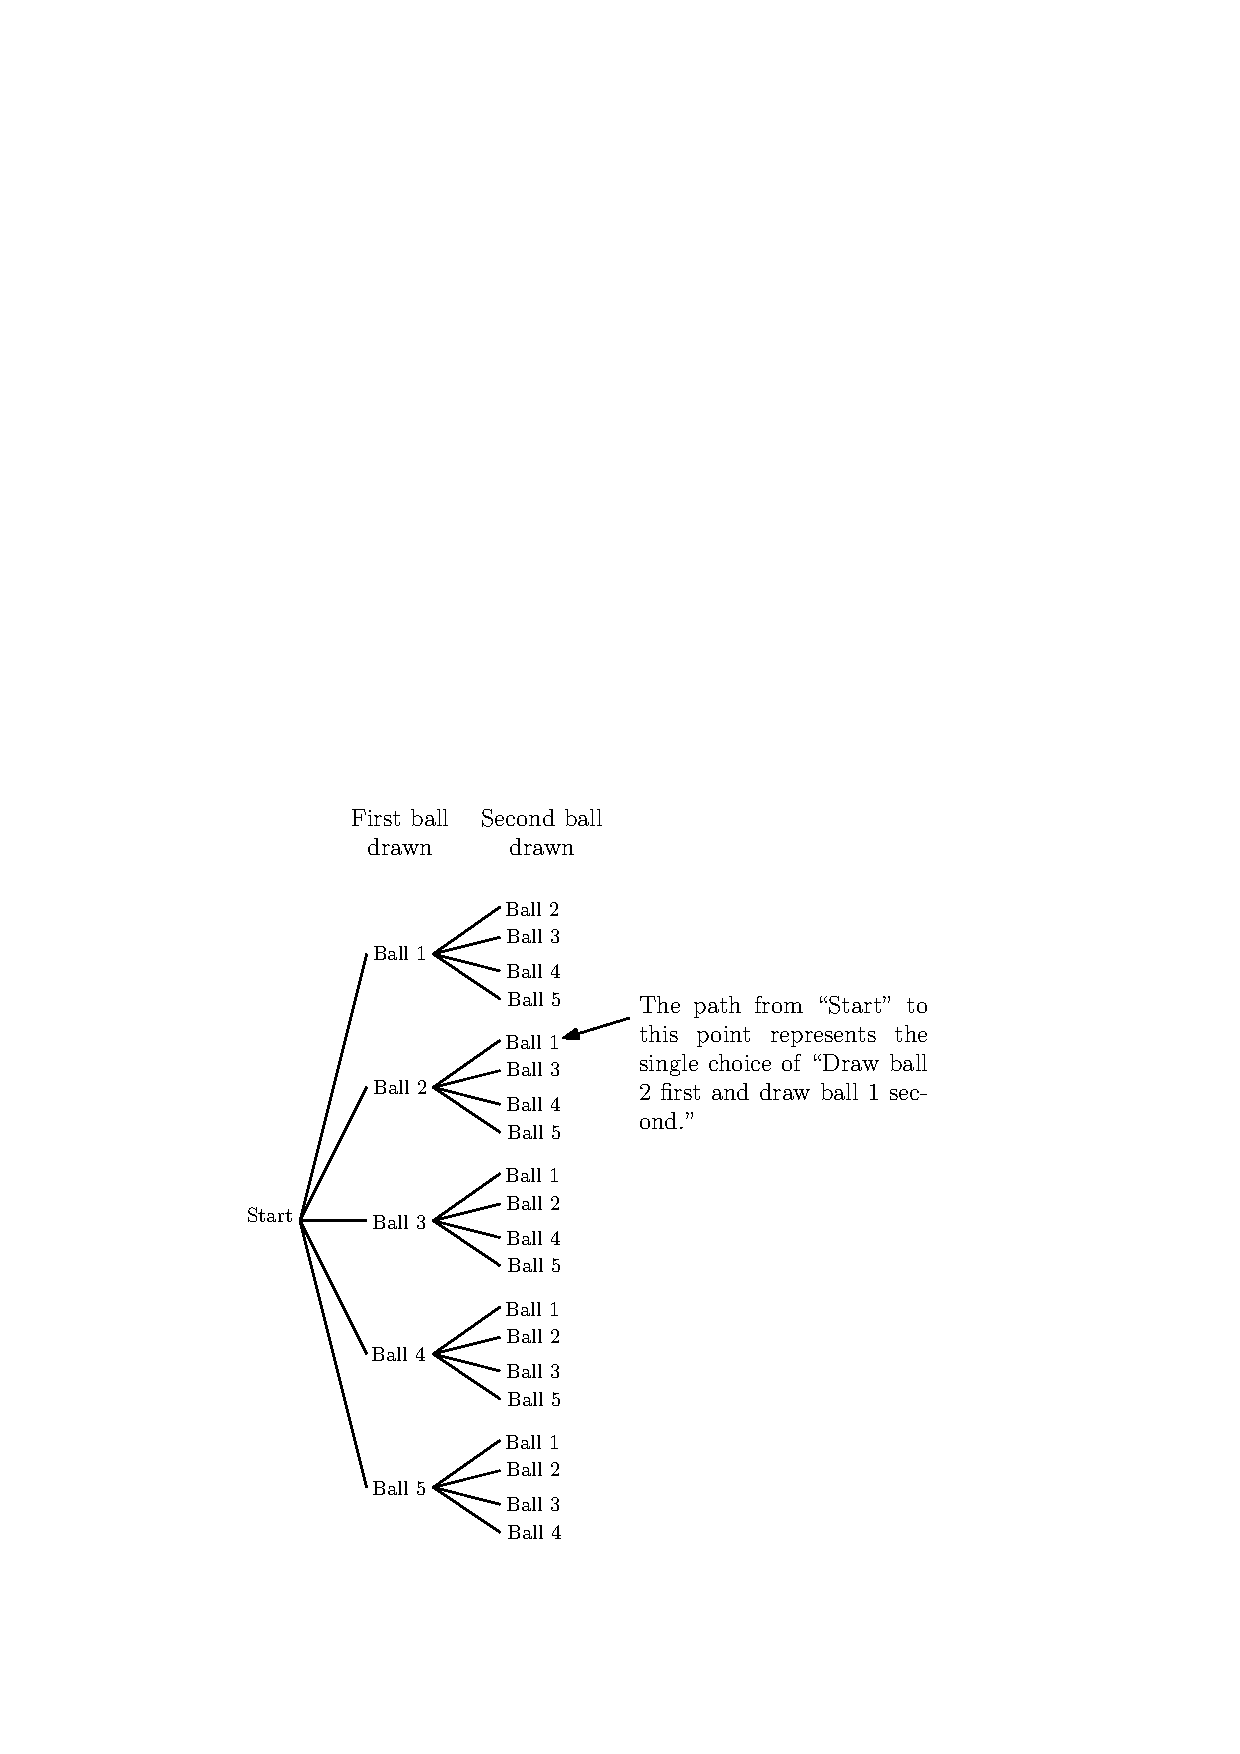
\includegraphics[width=3.5in]{images/raffleTree.pdf}
\end{center}
\caption{ $20$ different ways to draw two balls organized with a tree}\label{raffleTree}
\end{figure}
}

\wbvfill

%<*perm:raceselection:lotsWin>
\item\label{lotsWin} Lots of people started winning at the raffle, so Mario decides to make it more difficult for people to win. He starts the raffle over and increases the number of balls to eight (the eight balls are marked $1$, $2$, $3$, $4$, $5$, $6$, $7$, and $8$). Mario still draws two balls to determine the winners. Is it harder for participants to win? Explain your answer.
%</perm:raceselection:lotsWin>

\Instr{  This question is equivalent to asking, ``How many different ways are there to draw two balls when there are $8$ balls?'' There would be $8$ different options for the first draw, but the second draw would only have $7$ options. If we made a tree of the number of options, we have $7$ choices for the second ball for each of the $8$ possible ball choices during the first draw. So there are $8\times 7=56$ different possible drawings of two balls (without replacing the first ball).}
\end{enumerate}

\wbvfill

\wbnewpage


%%%%%%%%%  New Subsection  %%%%%%%%%%%%%%%%


\subsection{Activity: Raffles}
%<*perm:raceselection:stunt>
You want to be prepared in case Mario pulls a fast one on the participants again. So you and your buddies decide to determine how likely you are to win, no matter what number of balls are in the opaque box.
%</perm:raceselection:stunt>
\begin{enumerate}
%<*perm:raceselection:15balls>
\item If there are $15$ balls to choose from, how many possible balls are you able to choose during the first draw? How many balls remain after you remove the first chosen ball? So how many different ways are there to choose two balls (where the order in which they are chosen is important)?
%</perm:raceselection:15balls>

\Instr{  There are $15$ possible balls to pick during the first draw. After one ball has been chosen, there will only be $14$ left. So there are $15\times 14=210$ ways to select $2$ balls.}
\wbvfill


%<*perm:raceselection:20balls>
\item Say we have $20$ balls. So how many different ways are there to choose two balls (where the order in which they are chosen is important)?
%</perm:raceselection:20balls>

\Instr{  Similarly to the previous question, we have $20$ balls to choose from, but $19$ will remain after the first draw. So there are $20\times 19=380$ ways to select $2$ balls.}
\wbvfill

%<*perm:raceselection:nballs>
\item How many balls are available to be chosen for the first draw given $n$ balls? How many balls remain?  Explain your answer.
%</perm:raceselection:nballs>

\Instr{  With only $n$ balls to choose from, the first draw will have $n$ possible balls to choose from. There are $n-1$ balls remaining because you chose to pick one and put it aside for the first draw.}
\wbvfill

%<*perm:raceselection:nballs2draws>
\item\label{nballs2draws} How many different ways can $2$ balls be chosen if Mario starts with $n$ balls? Explain your answer.
%</perm:raceselection:nballs2draws>

\Instr{  There would be $n\times (n-1)$ different outcomes.}
\wbvfill

\wbnewpage

%<*perm:raceselection:1000>
\item\label{1000}  If you would like there to be at least $1000$ different ways of choosing two balls, what would be the fewest number of balls you would need in the opaque box? Explain how you reached your answer.
%</perm:raceselection:1000>

\Instr{  There are $1056$ ways to draw two balls when there are $33$ balls in the concealed box. Since $n\times (n-1)$ is the number of ways to choose $2$ balls from a box (without replacing the first ball), we want to find $n$ when $n\times (n-1)=1000$. Notice that $n$ must be rounded up to get a satisfactory answer.}
\wbvfill

%<*perm:raceselection:numDraws>
\item\label{numDraws} If you would like there to be at least $1000$ different ways of drawing $n$ balls, what would be the fewest number of draws you would need if there were $7$ balls in the opaque box?
%</perm:raceselection:numDraws>

\Instr{ 
With each successive draw there would be one less number of balls to choose from. So the number of different ways of drawing $n$ balls is $7\times 6\times\cdots \times (7-n)$. So we would need $5$ draws to get $7\times 6\times 5\times 4\times 3=2520$ different ways of drawing $5$ balls.
}
\wbvfill

%<*perm:raceselection:replace>
\item How would your answer change in Questions~{\normalfont\ref{nballs2draws}} and {\normalfont\ref{1000}} if the first ball drawn is replaced before the second is drawn?
%</perm:raceselection:replace>

\Instr{ 
After each ball is drawn there are still $n$ choices remaining, so we can use the Fundamental Counting Principle\index{Fundamental Counting Principle} to show there are $n\times n=n^2$ possible ways to draw $2$ balls from the concealed box.

To find the number of balls needed to have at least $1000$ different ways of drawing $2$ balls, we would solve $n\times n=n^2=1000$ for $n$ and round the answer up, so we would need $32$ balls in the concealed box.
}
\wbvfill

\end{enumerate}
\wbnewpage

%<*perm:raceselection:moreballs>
\indent Mario decides to be far sneakier than before. He will draw more than $2$ balls during the raffle. Each time he draws a ball, he will set it aside before drawing the next ball.
%</perm:raceselection:moreballs>

\begin{enumerate}
%<*perm:raceselection:10balls>
\setcounter{enumi}{7}
\item\label{10balls} If Mario starts with $10$ balls, how many balls remain after the $2^{nd}$ draw? So how many different ways are there to draw three balls (where the order in which they are chosen is important)?
%</perm:raceselection:10balls>

\Instr{  Since there would be $8$ balls remaining after removing the $2^{nd}$ ball, there are $8$ balls available. So there are $10\times 9 \times 8=720$ ways to select $3$ balls.}
\wbvfill

%<*perm:raceselection:tenballs1000>
\item  If Mario only has $10$ balls, how many will he need to draw to make sure there are at least $1000$ ways to choose the balls? 
%</perm:raceselection:tenballs1000>

\Instr{  There are $5040$ ways to choose $4$ balls from $10$ balls with no replacement. It is easy to see from Question~{\normalfont\ref{10balls}} that $10\times 9\times 8 <1000$.}
\wbvfill

%<*perm:raceselection:tenballs>
\item\label{tenballs}If Mario starts with $10$ balls, how many balls do you have to choose from on the $10^{th}$ draw?
%</perm:raceselection:tenballs>

\Instr{  Notice that this says ``$\ldots$on the $10^{th}$ draw?'' So there would be $9$ balls removed before the start of the $10^{th}$ draw. That means, there is only $1$ ball left to choose from.}

\wbvfill


%<*perm:raceselection:11draw>
\item\label{11draw} If Mario starts with $10$ balls, how many balls do you have to choose from on the $11^{th}$ draw? So how many ways are there to have $11$ draws with $10$ balls?
%</perm:raceselection:11draw>

\Instr{  The students should quickly realize that there will be no balls to choose from on the $11^{th}$ draw.}

\wbvfill

\wbnewpage


%<*perm:raceselection:drawsTable>
\item You are given a box in which the number of balls is given in the first column of the following table. The second column lists how many balls you have to draw, the order of which they are drawn being important. In column $3$, list the number of different ways the balls can be drawn.
\begin{center}
\begin{tabular}{|c|c|c|}
\hline
Number of balls in the box & Number of balls to be drawn & Number of different ways \\
\hline
\hline
$5$ & $3$ &  \\
\hline
$6$ & $3$ &  \\
\hline
$n$ & $3$ & \\
\hline
$5$ & $4$ & \\
\hline
$5$ & $5$ &\\
\hline
$5$ & $6$ & \\
\hline
$n$ & $m$ (with $m \leq n$)&\\
\hline
\end{tabular}
\end{center}
%</perm:raceselection:drawsTable>

\Instr{ 
\begin{center}
\begin{tabular}{|c|c|c|}
\hline
Number of balls in the box & Number of balls to be drawn & Number of different ways \\
\hline
\hline
$5$ & $3$ & $5\times 4 \times 3=60$ \\
\hline
$6$ & $3$ & $6\times 5 \times 4=120$ \\
\hline
$n$ & $3$ & $n\times (n-1) \times (n-2)$ \\
\hline
$5$ & $4$ & $5\times 4 \times 3 \times 2=120$ \\
\hline
$5$ & $5$ & $5\times 4 \times 3\times 2 \times 1=120$\\
\hline
$5$ & $6$ & $0$\\
\hline
$n$ & $m$ (with $m\leq n$) & $n\times (n-1)\times \cdots \times(n-m+1)$\\
\hline
\end{tabular}
\end{center}
}

\end{enumerate}

\wbnewpage
%<*perm:SelectingaJury:title>
\subsection{Extension Activity: Selecting a Jury}\label{Selecting a Jury}
%</perm:SelectingaJury:title>

\Instr{  
Goals for this activity:
\begin{packedItem}
\item Using a list method to detremine the number of combination; and
\item developing a abstract formula for combinations.
\end{packedItem}
}


%%%%%%%%%  New Subsection  %%%%%%%%%%%%%%%%

\subsection*{Entrance Activity}

Imagine you are working in a small business with four people (say Alice, Bob, Charlie, and you) and many of the projects your business needs to complete require partners to work together. 

\begin{enumerate}
\item \label{YouPartners} How many different partners could you possible work with on a project? List all the partnerships you can be apart of.

\Instr{  Obviously there are three other people so you could be matched with any of the three people forming three different partnerships.

You and Alice are a partnership.

You and Bob are a partnership.

You and Charlie are a partnership.
}

\wbvfill

\item \label{AlicePartners} How many different partners could Alice work with on a project? List all the pairs of people containing Alice?

\Instr{  Again we have that Alice is apart of three pairs. Alice and Bob are a pair, Alice and Charlie are a pair, and Alice and you are a pair.
}

\wbvfill

\item \label{Partnerships} Do you see any pairs that show up in questions \ref{YouPartners} and \ref{AlicePartners}?

\Instr{  Here we should notice that the pair You and Alice appears in both Questions~\ref{YouPartners} and \ref{AlicePartners}.
}

\wbvfill

\item \label{ListAllPartnerships} List all the pairs of people that exist at your work.

\Instr{  All of the pairs that can be made are

\begin{center}
\begin{tabular}{c}
You and Alice \\
You and Bob \\
You and Charlie \\
Alice and Bob \\
Alice and Charlie \\
Bob and Charlie \\
\end{tabular}
\end{center}
}

\wbvfill

\end{enumerate}

\wbnewpage


%%%%%%%%%  New subSection  %%%%%%%%%%%%%%%%

\subsection{Jury Duty}


\indent The small town of \town has experienced its first felony. The deputies' office has apprehended a suspect and Mayor Catie wants him to stand trial in their very own courtroom. She has gathered $7$ citizens for jury selection: {\bf A}lice, {\bf B}ob, {\bf C}harlie, {\bf D}oug, {\bf E}rika, {\bf F}red, and {\bf G}eorge.  Of those $7$, the mayor needs to pick $3$ to sit on the jury. To make the selection process fair, for each possible combination of $3$ people selected from these $7$ citizens in turn, she writes the names of the $3$ people on a sheet of paper. She places all the sheets of paper in a box and then selects one piece of paper. The people with names on the selected piece of paper become the jury. Your job is to determine how many pieces of paper she will need so that all possible juries are placed into the box.
%</perm:SelectingaJury:intro>
\begin{enumerate}
%<*perm:SelectingaJury:combolist>
 \item\label{combolist} Describe several methods to make a list of the possible juries. Make sure your methods do not miss nor duplicate any juries!
%</perm:SelectingaJury:combolist>

\Instr{  Students should think of ways to list out each combination\index{combination}. For example, they could make an alphabetical listing using the first letters of each person's name. They may come up with some other technique. Using a tree diagram\index{tree diagram} works well, and could be encouraged. See Question~{\normalfont\ref{organization}} for the list of all the different possible juries of size $3$ from $7$ people.}

\wbvfill

%<*perm:SelectingaJury:comboproc>
 \item\label{comboproc} Which of your lists from Question~{\normalfont\ref{combolist}} is organized in a way that is easy to count? If none, come up with a way to organize the list so it is easy to count.
%</perm:SelectingaJury:comboproc>

\Instr{  Here they may want to group the juries together which have certain properties. One example is to begin by listing all the juries that include the first person. This gives rise to a recursive procedure, because the only juries left to count are all the juries that can be made from the remaining $6$ people.}
\wbvfill

%<*perm:SelectingaJury:organization>
 \item\label{organization} Is each jury represented through the organization process given in Question~{\normalfont\ref{comboproc}}? Explain your results. List all the possibilities, choosing an approach that makes it clear that each $3$-person jury is included exactly once. How many juries did you find?
%</perm:SelectingaJury:organization>

\Instr{  The students should now check to make sure they have not missed any possible combinations\index{combination} (juries). Also verify that the organization process does produce each possible outcome. Table~{\normalfont\ref{comboLetters}} gives one such list of the $35$ possible juries using the first letters of each of their names.
\renewcommand{\thetable}{\arabic{chapter}.\arabic{table}(\alph{bluetable})} 
% \setcounter{bluetable}{1}
\addtocounter{table}{-1}
\addtocounter{bluetable}{1}
\begin{table}[htb]
\inst
\begin{center}
\begin{tabular}{ccccccccc}
ABC && BCD && CDE && DEF && EFG \\
ABD && BCE && CDF && DEG && \\
ABE && BCF && CDG && DFG && \\
ABF && BCG && CEF && && \\
ABG && BDE && CEG && &&  \\
ACD && BDF && CFG &&  && \\
ACE && BDG && &&  &&  \\
ACF && BEF && &&   && \\
ACG && BEG && &&  &&  \\
ADE && BFG && &&   && \\
ADF && &&  &&   && \\
ADG && &&  &&  &&  \\
AEF && &&  &&   && \\
AEG && &&  &&  &&  \\
AFG && &&  &&  &&  \\
\end{tabular}
\end{center}
\caption{A list of all possible seatings using the first letters of each name}\label{comboLetters}
\end{table}

The students may notice that the number of entries in each column matches the number of rectangles in a $1\times n$ array they found in Activity~{\normalfont\ref{recursion}}. You could challenge the students to find a reason why they are the same. For example, to use rectangles to count the number of entries in the first column of Table~{\normalfont\ref{comboLetters}}, start by recognizing that they all contain A, so only the other two letters must be chosen. Assign those $6$ letters to the $6$ cells in the $1\times 6$ array:
\renewcommand{\thefigure}{\arabic{chapter}.\arabic{figure}(\alph{bluefigure})} 
%  \setcounter{bluefigure}{1}
\addtocounter{figure}{-1}
\addtocounter{bluefigure}{1}
\begin{figure}[H]
\begin{center}
\begin{tabular}{cccccc}
B & C & D & E & F & G \\
\hline
\multicolumn{1}{|c}{} & \multicolumn{1}{|c}{} & \multicolumn{1}{|c}{} & \multicolumn{1}{|c}{} & \multicolumn{1}{|c}{} & \multicolumn{1}{|c|}{} \\
\hline
\end{tabular}
\end{center}
\caption{$1\times 6$ array}\label{1by7array}
\end{figure}
Each rectangle produces one of the combinations (juries) in the first column by using the names of the first and last cell in the chosen rectangle together with letter A. For example, the highlighted rectangle Figure~{\normalfont\ref{AtoCE}} produces the jury ACE.
\renewcommand{\thefigure}{\arabic{chapter}.\arabic{figure}(\alph{bluefigure})} 
%  \setcounter{bluefigure}{1}
\addtocounter{figure}{-1}
\addtocounter{bluefigure}{1}
\begin{figure}[htb]
\begin{center}
\begin{tabular}{cccccc}
B & C & D & E & F & G \\
\hline
\multicolumn{1}{|c}{} & \multicolumn{1}{|c}{\cellcolor{gray}} & \multicolumn{1}{|c}{\cellcolor{gray}} & \multicolumn{1}{|c}{\cellcolor{gray}} & \multicolumn{1}{|c}{} & \multicolumn{1}{|c|}{} \\
\hline
\end{tabular}
\end{center}
\caption{Example of choosing a jury that includes Alice}\label{AtoCE}
\end{figure}
}

\wbvfill

\wbvfill


\wbnewpage


%<*perm:SelectingaJury:3outof10>
\item\label{3outof10} If the mayor had to choose $4$ people for the jury from the $7$ people, how many juries could be formed? Is there some relationship between your answer to this question and the number of possibilities you gave in Question~{\normalfont\ref{organization}}?
%</perm:SelectingaJury:3outof10>

\Instr{  
There are $35$ possible juries that contain $4$ people.

Here the students should recognize this is the same number of combinations (juries) as when choosing $3$ jurors. You may want to ask the students 

\begin{minipage}[H]{5.75in}
\tt \em
\begin{center}
``If ABC are on the jury, who is at home?''

 ``Is there any other jury where these same people are at home?''

``Why may this be true?''
\end{center}
\end{minipage}

Each combination\index{combination} of $3$ jurors left out $4$ of the $7$, so another way to look at this is to count each combination as those that were left out. Here we see it is obvious that selecting $3$ jurors produces the same number of combinations as selecting $4$ jurors.}

\wbvfill

%\vspace{.4in}
%<*perm:SelectingaJury:allcombinations>
\item\label{allcombinations} For the future, we would like to know how many possible juries there are when picking any number of jurors from $7$ people. So if we have a pool of $7$ people from which to choose, fill in the table below.
\begin{center}
\begin{tabular}{|c|c|}
\hline
Number of people in jury & Number of different juries \\
\hline
\hline
$1$ & \\
\hline
$2$ & \\
\hline
$3$ & \\
\hline
$4$ & \\
\hline
$5$ & \\
\hline
$6$ & \\
\hline
$7$ & \\
\hline
\end{tabular}
\end{center}
%</perm:SelectingaJury:allcombinations>

\Instr{  Hopefully the students will find some easy methods to listing and organizing the possible juries. Also with the relationship established in Question~{\normalfont\ref{3outof10}}, they should know that selecting $1$ person is the same as selecting $6$ people, selecting $2$ people is the same as selecting $5$ people, and selecting $3$ people is the same as selecting $4$ people. 
\begin{center}
\begin{tabular}{|c|c|}
\hline
Number of people in jury & Number of different juries \\
\hline
\hline
$1$ & $7$ \\
\hline
$2$ & $21$ \\
\hline
$3$ & $35$ \\
\hline
$4$ & $35$ \\
\hline
$5$ & $21$ \\
\hline
$6$ & $7$ \\
\hline
$7$ & $1$ \\
\hline
\end{tabular}
\end{center}
}

%<*perm:SelectingaJury:permutation>
\end{enumerate}

\wbnewpage

Mayor Catie was thinking about the number of $3$-person juries she could select from the pool of $7$ people: {\bf A}lice, {\bf B}ob, {\bf C}harlie, {\bf D}oug, {\bf E}rika, {\bf F}red, and {\bf G}eorge. She really wanted to make use of her preference for using permutations whenever possible. After all, sitting next to the window in the jury box might be a desirable seat!

\begin{enumerate}
\setcounter{enumi}{5}
\item\label{permutation} What would happen to the number of different juries if the jury selected is to be seated in a certain order? For example, if Alice sits in the left seat, Bob sits in the middle seat and Charlie sits in the right seat, it is a different jury to if Bob sits in the left seat, Alice sits in the middle seat and Charlie sits in the right seat. How many different {\em ordered} jury seatings are there if $3$ jurors out of $7$ people are to be seated?
%</perm:SelectingaJury:permutation>

\Instr{  It may not be obvious to the students, but this question is the same type of problem as in Activity~{\normalfont\ref{raceselection}}. It may help the students to ask 

\begin{minipage}[H]{5.75in}
\tt \em
\begin{center}
{``Can we use some method we used in a previous activity?''}
\end{center}
\end{minipage}

The answer to this question is ${}_7P_3=7\times 6 \times 5=210$. So introducing an order into the selection moves us from combinations\index{combination} back to permutations\index{permutation}. The aim with this question is two fold: to help students see the difference between permutations\index{permutation} and combinations and to eventually show how permutations can be used to count the number of combinations (see Question~{\normalfont\ref{questions678}}).
}

\wbvfill

%<*perm:SelectingaJury:repeats>
\item\label{repeats} Suppose Alice, Bob, and Charlie are selected to sit on the jury. How many ways are there to seat these $3$ jurors if the order in which they are seated matters?
%</perm:SelectingaJury:repeats>

\Instr{  The students could use a tree to see which seatings involve Alice, Bob, and Charlie? Also, they could list out all the different permutations.\index{permutation} Both approaches are important. 

There are $6$ different ways to seat Alice, Bob, and Charlie:
\begin{center}
\begin{tabular}{ccccc}
ABC && BAC && CAB \\
ACB && BCA && CBA \\
\end{tabular}
\end{center}
}

\wbvfill

%<*perm:SelectingaJury:seatingarrangements>
\item\label{seatingarrangements} Does the number of seated juries found in Question~{\normalfont\ref{repeats}} change if we have a different set of three jurors? Explain your answer.
%</perm:SelectingaJury:seatingarrangements>

\Instr{  Regardless of which $3$ jurors we are considering, there are always $6$ combinations for their seating arrangements. The reason that the number does not change is because the possible orders they can sit is not dependent on which three jurors have been selected.}

\wbvfill

%<*perm:SelectingaJury:questions678>
\item\label{questions678} Return to Question~{\normalfont\ref{organization}} where we found the number of juries of $3$ people that Mayor Catie can choose from $7$ people when the order in which they sit does \emph{not} matter. How can you use the answers to Questions~{\normalfont\ref{permutation}}, {\normalfont\ref{repeats}}, and {\normalfont\ref{seatingarrangements}} above to find this number? ({\em Hint}: Think about how many times each unordered jury is counted in your answer to Question~{\normalfont\ref{permutation}}.)
%</perm:SelectingaJury:questions678>

\Instr{  This is a critical observation and worth thoroughly exploring. After the students have had some time to think about the problem, you may want to introduce the following question.

\begin{minipage}[H]{5.75in}
\tt \em
\begin{center}
{``If a little ant was walking around the room counting people, how might the ant do it?''}
\end{center}
\end{minipage}

\noindent Usually someone will suggest counting all the legs. Then what? Divide the number of legs by two. It is easier for the ant to over count, but count each object of interest (i.e. the people) the same number of times (i.e. twice). Then ask

\begin{minipage}[H]{5.75in}
\tt \em
\begin{center}
{``How does the ant count the number of chairs?''}
\end{center}
\end{minipage}

\noindent Count the legs and divide by $4$ is the answer you hope to get.

This approach is relevant here because Question~{\normalfont\ref{permutation}} tells the students how many possible juries there are if the order in which the jury sits matters. Question~{\normalfont\ref{repeats}} tells the students how many possible juries there are with just Alice, Bob, and Charlie when the order in which they sit matters. Question~{\normalfont\ref{seatingarrangements}} tells the students that the number of juries produce with just Alice, Bob, and Charlie found in Question~{\normalfont\ref{repeats}} is the same for any $3$ jurors. So we have over counted the number of juror seatings in Question~{\normalfont\ref{permutation}}; but Question~{\normalfont\ref{repeats}} says this over count in fact counts each jury (if we disregard the order) the same number of times, namely $6$ times. By dividing the total number of juries where the seating order does matter by the number of times the same three people are seated provides the total number of juries where the seating order does not matter: $210/6=35$.
}
\end{enumerate}

\wbvfill

\wbnewpage

%<*perm:SelectingaJury:mayorselects>
Let us try to determine what could happen in any situation. So assume that the mayor needs to select a jury of $r$ people from a population of $n$ people. The mayor does not care where they sit, but at first we will! So assume that we have $r$ seats in a row, numbered $1$ to $r$ from left to right. We will start by seeing how many seating arrangements we can have, then group them by which seating arrangements have selected the same group of jurors.
%</perm:SelectingaJury:mayorselects>
\begin{enumerate}
%<*perm:SelectingaJury:firstpick>
\setcounter{enumi}{9}
\item For the first seat how many people are available to be chosen to sit in this seat? 
%</perm:SelectingaJury:firstpick>

\Instr{  We can choose any of the $n$ people.}
\wbvfill
%<*perm:SelectingaJury:secondpick>
\item After we have chosen our first person, how many people are available to be chosen for our second seat? 
%</perm:SelectingaJury:secondpick>

\Instr{  We can pick any person not already chosen, so $n-1$ people.}
\wbvfill
%<*perm:SelectingaJury:ithpick>
\item\label{iChair} So for the $i^{th}$ chair, how many people are available to be chosen? 
%</perm:SelectingaJury:ithpick>

\Instr{  It may help to form a table comparing the number of people available to be chosen to the number of chairs that are filled. (See Table~{\normalfont\ref{peopleAvailable}} for an example.)

To seat the next juror, we need to select $1$ person from the people which have not yet been chosen. Since $i-1$ people have already been chosen, we have $n-(i-1)$ or $n-i+1$ options for the next juror. This generalizes the counting in Question~{\normalfont\ref{permutation}}.
\renewcommand{\thetable}{\arabic{chapter}.\arabic{table}(\alph{bluetable})} 
% \setcounter{bluetable}{1}
\addtocounter{table}{-1}
\addtocounter{bluetable}{1}
\begin{table}[htb]
\inst
\begin{center}
\begin{tabular}{|c||c|c|c|c|c|c|c|c|c|}
\hline
Number of people  & \multirow{2}{*}{$n$} & \multirow{2}{*}{$n-1$} & \multirow{2}{*}{$n-2$} & \multirow{2}{*}{$\cdots$} & \multirow{2}{*}{$n-i+1$} & \multirow{2}{*}{$n-i$} & \multirow{2}{*}{$\cdots$} & \multirow{2}{*}{$1$} & \multirow{2}{*}{$0$}\\
not seated on jury & &&&&&&&& \\
\hline
Number of chairs & \multirow{2}{*}{$0$} & \multirow{2}{*}{$1$} & \multirow{2}{*}{$2$} & \multirow{2}{*}{$\cdots$} & \multirow{2}{*}{$i-1$} & \multirow{2}{*}{$i$} & \multirow{2}{*}{$\cdots$} & \multirow{2}{*}{$n-1$} & \multirow{2}{*}{$n$} \\
containing a juror &&&&&&&&& \\
\hline
\end{tabular}
\end{center}
\caption{Number of people available to be chosen for the following chair on the jury based on how many chairs on the jury have been filled}\label{peopleAvailable}
\end{table}
}
\wbvfill
%<*perm:SelectingaJury:total>
\item\label{perm:SelectingaJury:total} Can you use the approach used in Questions~{\normalfont\ref{repeats}} and {\normalfont\ref{seatingarrangements}} to count the total number of options to seat $r$ jurors in precisely $r$ seats where the order in which they sit does matter? 
%</perm:SelectingaJury:total>

\Instr{  We can apply the Fundamental Counting Principle in Chapter~{\normalfont\ref{chap1}} and the discussion about permutations\index{permutation} from Activity~{\normalfont\ref{raceselection}}. So the answer is obtained by multiplying $r$ the $r$ integers from $r$ to $1$, namely $r!$ (this generalizes the counting in Questions~{\normalfont\ref{seatingarrangements}} and {\normalfont\ref{questions678}}).}
\wbvfill
%<*perm:SelectingaJury:nomatch>
\item Can you use the answers to Questions~{\normalfont\ref{iChair}} and {\normalfont\ref{perm:SelectingaJury:total}} to count the number of juries with $r$ people that can be chosen from a group of $n$ people where the order in which they sit is irrelevant?
%</perm:SelectingaJury:nomatch>

\Instr{  This question generalizes the counting approach in Question~{\normalfont\ref{perm:SelectingaJury:total}}. Here we make the observation that two outcomes counted by using the Fundamental Counting Principle could possibly involve precisely the same group of people, just seated in a different order; we have been counting permutations\index{permutation}. So we have over counted. 

We notice that the over counting actually counts each group (combination) of people exactly $r!$ times. So we can divide our number of permutations by the number of times we counted each group to find the number of  juries with $r$ people. This can be written as
$$\frac{n(n-1)(n-2)\cdots(n-r+1)}{r!}=\frac{n!}{r!(n-r)!}.$$
}
\wbvfill
%<*perm:SelectingaJury:devise>
\item Can you devise a way which accurately gives the number of possible juries without listing all combinations\index{combination}? Test your hypothesis on finding the number of combinations selecting $3$ jurors from $8$ people.
%</perm:SelectingaJury:devise>

\Instr{  As we said, we over count by the number of permutations\index{permutation}. So we can divide by this number to get an accurate number of possible juries. The formula is ${}_n C_r=\binom{n}{r}=\frac{{}_nP_r}{r!}=\frac{n!}{r!(n-r)!}$.}

\end{enumerate}
\wbvfill

\wbnewpage
%%%%%%%%%%%%%%%%%%%%%%%%%%%%%%%%%%%%%%%%
%%%%%%%%%  New Section  %%%%%%%%%%%%%%%%
%%%%%%%%%%%%%%%%%%%%%%%%%%%%%%%%%%%%%%%%
\section{Shipping Candy}


%%%%%%%%%  New Subsection  %%%%%%%%%%%%%%%%

\subsection{Entrance Activity: It's time for a break!}
\begin{center}
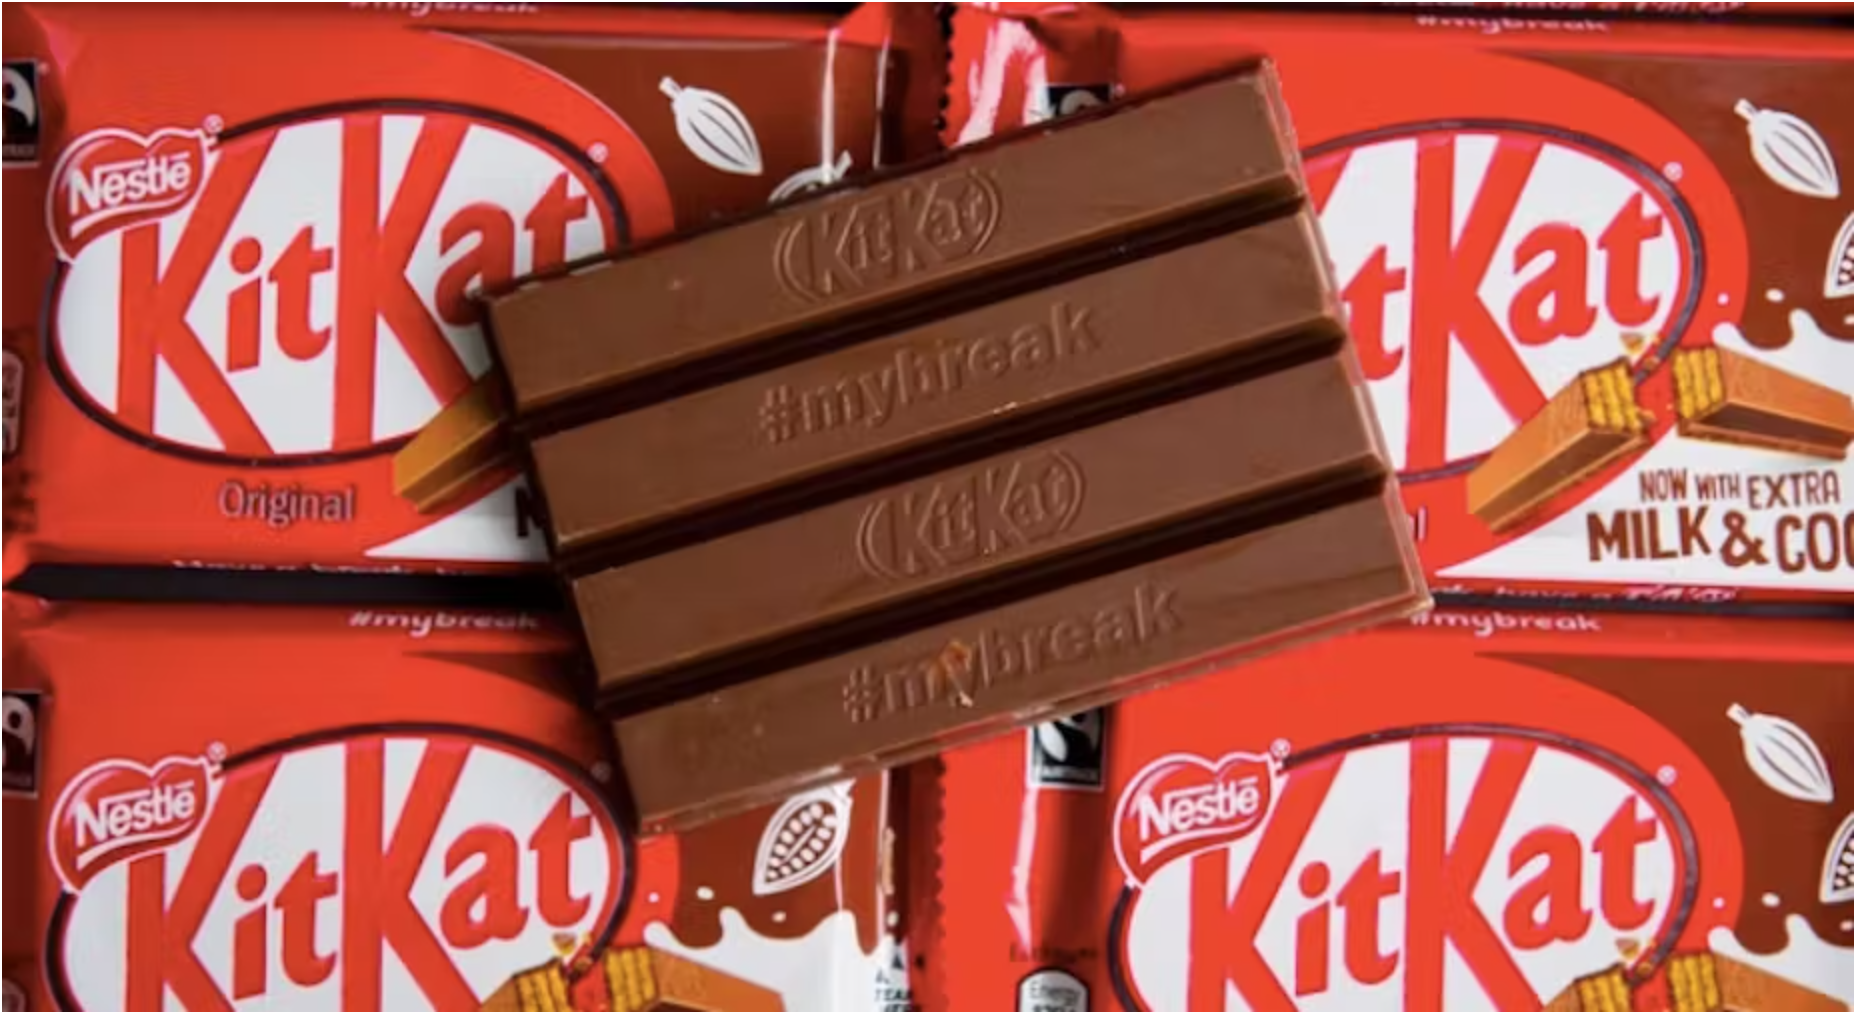
\includegraphics[scale =0.25]{images/KitKat.png}
\end{center}

A KitKat package comes with four individual wafer bars as shown in the image above.

\begin{enumerate}
    \item How many wafer bars are there in 4 KitKat packages?
    
    \wbvfill
    
    
    \item If you have 97 wafer bars, how many \textbf{complete} KitKat packages could you have?
    
    \wbvfill
    
    \wbvfill
\end{enumerate}

\wbnewpage

%%%%%%%%%  New Subsection  %%%%%%%%%%%%%%%%

\subsection{Activity: How many can we pack in a Shipment?}
You are charged with filling and invoicing store shipment orders of KitKat to individual convenience stores across the country. For some reason the website for purchasing is set up to request the number of wafers a store wishes to purchase.

\begin{enumerate}
    \item You cannot ship individual wafers as each must be sealed into a package, so which of the following stores are you able to fill an order for?
    \begin{enumerate}
        \item Store A has ordered $368$ wafers
        \wbvfill
        \item Store B has ordered $528$ wafers
        \wbvfill
        \item store C has ordered $12,346$ wafers
        \wbvfill
    \end{enumerate}
    
    \item Can you describe an easy way to determine if the order can be filled?
    \wbvfill
\end{enumerate}
\wbnewpage
To invoice the stores for shipping you need to figure out the total cost to your company. Obviously buying in bulk will be helpful to stores but packaging and shipping varies depending on the exact order as described below.

\begin{itemize}
    \item A single package of KitKats cost \$0.72 to package and ship.
    \item A sleeve of KitKats consists of four packages and costs \$1.54 to package and ship.
    \item A carton of KitKats consists of four sleeves and costs \$3.18 to package and ship.
    \item A box of KitKats consists of four cartons and costs \$6.46 to package and ship.
    \item A crate of KitKats consists of four boxes and costs \$13.02 to package and ship.
\end{itemize}

For example, if a store ordered 20 wafer bars, that would be packaged and shipped in the containers of one sleeve and one package to minimize cost. The total cost for shipping this way is \$1.54 + \$.72 = \$2.26. Your job is to make sure your orders are shipping for the lowest cost.

\begin{enumerate}\setcounter{enumi}{2}
    \item How many wafers are in 2 cartons and 3 sleeves?
    \wbvfill
    \item How many wafers are in 1 crate?
    \wbvfill
    \item How many wafers are in 2 boxes, 3 cartons, 1 sleeve, and 1 package? How much does it cost to ship these wafers?
    \wbvfill
    \wbnewpage
    \item In what packaging containers would you ship 56 wafer bars? How much would that cost? Remember, you are trying to ship them at minimum cost.
    \wbvfill
    \item In what packaging containers would you ship 156 wafer bars? How much would that cost?
    \wbvfill
    \item Al owns three convenience stores and realizes he can save money if he has all three of his orders combined into one. He calls to ask this after you have calculated each of his shipments, which are each listed below. Can you figure out his combined order without counting the number of individual wafers ordered?
    \begin{itemize}
        \item Store 1: 1 box, 2 cartons, 3 sleeves and 1 package.
        \item Store 2: 3 cartons and 3 packages.
        \item Store 3: 2 boxes, 2 cartons, and 2 sleeves.
    \end{itemize}
    
    \wbvfill
    
    \wbvfill
\end{enumerate}

\wbnewpage
You have obviously impressed your bosses with your money saving acumen. You have been promoted to manager in charge of all candy distribution!

\begin{center}
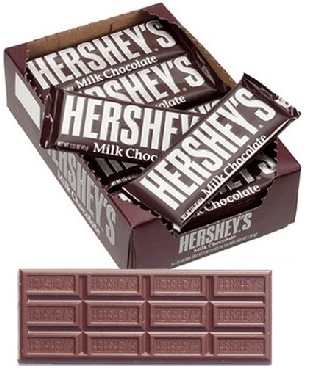
\includegraphics[scale =0.5]{images/Hershey.png}
\end{center}

Hershey bars are packaged in groups of 12 and shipped by the following requirements:
\begin{itemize}
    \item A single package of Hershey cost \$0.12 to package and ship.
    \item A box of Hershey consists of twelve packages and costs \$1.30 to package and ship.
    \item A carton of Hershey consists of twelve boxes and costs \$12.50 to package and ship.
    \item A crate of Hershey consists of twelve cartons and costs \$140.75 to package and ship.
\end{itemize}
\begin{enumerate}\setcounter{enumi}{8}
    \item How many Hershey pieces are in 1 crate?
    \wbvfill
    \item How many Hershey pieces are in 2 cartons, 11 boxes, and 5 packages? How much does it cost to ship these pieces?
    \wbvfill
    \wbnewpage
        \item In what packaging containers would you ship 1,020 Hershey pieces? How much would that cost?
    \wbvfill
    \item In what packaging containers would you ship 3,744 Hershey pieces? How much would that cost?
    \wbvfill
    \item Al calls to combine his three orders. Without calculating the total number of individual pieces or packages ordered what is the total shipment packaging and what does it cost?
    \begin{itemize}
        \item Store 1: 10 cartons, 8 boxes and 11 packages.
        \item Store 2: 5 cartons and 9 packages.
        \item Store 3: 2 crates, 7 cartons, and 2 boxes.
    \end{itemize}
    
    \wbvfill
    
    \wbvfill
\end{enumerate}
\wbnewpage

\subsection{Exit Activity: Caramello Bars}


\begin{center}
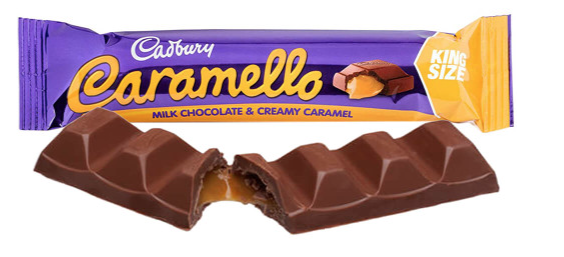
\includegraphics[scale =0.5]{images/Caramello.png}
\end{center}

As you can see Caramellos are packaged in groups of 6. They are shipped by the following requirements:
\begin{itemize}
    \item A single package of Caramellos cost \$0.15 to package and ship.
    \item A sleeve of Caramellos consists of six packages and costs \$0.85 to package and ship.
    \item A box of Caramellos consists of six sleeves and costs \$4.50 to package and ship.
    \item A crate of Caramellos consists of six boxes and costs \$24.75 to package and ship.
\end{itemize}
\begin{enumerate}
    \item How many Caramellos are there in 5 boxes, 4 sleeves, and 3 packages?
    \wbvfill
    \item In what packaging containers would you ship 270 Caramellos? How much would that cost?
    \wbvfill
\end{enumerate}
\wbnewpage
\noindent For sake of efficiency, the candy shipping company uses an abbreviation for each shipment. They simply list the number of crates, boxes, sleeves, packages, and individual Caramellos to be sent using a sequence of digits, in that order. For example, a shipment of 5 crates, 3 boxes, and 4 packages would be abbreviated as 53040. Notice the third digit is 0 since zero sleeves are being sent, and there will always be a 0 at the end since, at this time, individual Caramellos cannot be shipped.
\begin{enumerate}[resume]
	\item How many individual Caramellos, packages, sleeves, boxes, and crates are sent in the order abbreviated by 20450?
    \wbvfill
    \item How many Caramellos, in total, are sent in the order abbreviated by 20450?
    \wbvfill
    \item What would be the abbreviation for the least expensive shipment of 1000 Caramellos?
    \wbvfill
\end{enumerate}

\wbnewpage

%%%%%%%%%%%%%%%%%%%%%%%%%%%%%%%%%%%%%%%%
%%%%%%%%%  New Section  %%%%%%%%%%%%%%%%
%%%%%%%%%%%%%%%%%%%%%%%%%%%%%%%%%%%%%%%%
%\section{Binary - the language of computers} % Need to add this section


%%%%%%%%%%%%%%%%%%%%%%%%%%%%%%%%%%%%%%%%
%%%%%%%%%  New Section  %%%%%%%%%%%%%%%%
%%%%%%%%%%%%%%%%%%%%%%%%%%%%%%%%%%%%%%%%
\section{Counting Rhythm}


%%%%%%%%%  New Subsection  %%%%%%%%%%%%%%%%

\subsection{Entrance Activity: Writing Rhythm}

Music is the beautiful embodiment of patterns in sound. While there are enough connections between mathematics and music to create an entire course, we will explore just one connection by looking at rhythm. 

Listen to the clip at \href{https://www.youtube.com/watch?v=SnjqxgtLJlA}{https://www.youtube.com/watch?v=SnjqxgtLJlA}. In the background of the audio you hear a small ticking that is keeping track of ``time" or ``counting time." The first four ticks are just meant as introduction as the music starts on the fifth tick. Find a way to describe on which ticks the musician plays his instrument and which he does not. Use this method to describe the entire sequence of rhythm played in the video.

\newpage

%%%%%%%%%  New Subsection  %%%%%%%%%%%%%%%%
\subsection{Activity: Exploration of Rhythm}

Begin by discussing how each member of your group denoted the rhythm played in the video. 
\begin{enumerate}
    \item Come to a consensus in your group for how you will write down a rhythm and re-write the rhythm from the video here.
    \wbvfill
    \item Does the rhythm repeat itself, and if so how long does it take to begin repeating? Write down the shortest length of rhythm that is then continuously repeated? (Hint: professionals would say this rhythm has 3 beats (and 5 rests) within an eight count.
    \wbvfill
\end{enumerate} 
    
 We want to know how many different rhythms exist. As a common strategy, let's start with a small number of counts and see if we can find all the rhythms in the world. To make things uniform we will use a ``1'' to indicate a beat and a ``0'' to indicate a rest. For instance the beat you heard in the on-line clip is 10010010.
 \begin{enumerate}\setcounter{enumi}{2}
    \item Can you list a different rhythm with 3 beats within an eight count?
    \wbvfill
    \item John plays three ``rounds'' of your rhythm. So write the rhythm as 24 counts by repeating the eight count rhythm twice.
    \wbvfill
    \item Imagine someone didn't hear the first three beats of John playing your rhythm. What might they say was the eight count rhythm? Is this the same rhythm or different? 
    \wbvfill
\end{enumerate}

\wbnewpage

\subsection{Activity: Finding Your Rhythm}

Let's see if we can't find all the rhythms that exist, this may be a bit difficult, but we can at least try!

\begin{enumerate}

\item \label{2/4rhythm}Can you list out all the rhythms with 2 beats on four counts? Think about how you can organize this list to get all of them. (Yes actually list them all!)

\wbvfill
\item \label{3/4rhythm} Now list all the rhythms with 3 beats on four counts?
\wbvfill
\item Imagine you have listened to the first four counts of a five count rhythm. What are the possibilities for the last count? If you knew how many beats were in the rhythm at the beginning, would you be able to guess what the last count would be after listening to the first four counts?
\wbvfill
\item How can the answers from questions \ref{2/4rhythm} and \ref{3/4rhythm} help you to all the rhythms on five counts with 3 beats?
\wbvfill

\wbnewpage
\item Below are the list of all three count rhythms. How can you build on these to create the rhythms you listed in questions \ref{2/4rhythm}?

\begin{tabular}{ccc}
    $000$ & $100$ & $010$ \\
     $001$ & $110$ & $011$\\
     $101$ & $111$ &
\end{tabular}

\wbvfill

\item Can you quickly fill out the entire table below? Describe the process you are using.

\begin{tabular}{|c|c|c|c|c|c|c|c|c|}
\hline
     & 0 beats & 1 beats & 2 beats & 3 beats & 4 beats & 5 beats & 6 beats & 7 beats \\
     \hline
     2 counts &&&&&&&& \\
      \hline
     3 counts &&&&&&&& \\
      \hline
     4 counts &&&&&&&& \\
      \hline
     5 counts &&&&&&&& \\
      \hline
     6 counts &&&&&&&& \\
      \hline
     7 counts &&&&&&&& \\
      \hline
\end{tabular}

\wbvfill
\end{enumerate}


\newpage

%%%%%%%%%%%%%%%%%%%%%%%%%%%%%%%%%%%%%%%%
%%%%%%%%%  New Section  %%%%%%%%%%%%%%%%
%%%%%%%%%%%%%%%%%%%%%%%%%%%%%%%%%%%%%%%%
\section{Project Choices}

\begin{enumerate}
\item \textbf{Fundamental Counting Principle \& Dependent Choices:} While we generally say that the fundamental counting principle can only be used when working with  independent "choices" provide an example of a situation (not used in class!) where one can use the fundamental counting principle to count the number of outcomes in a situation that has dependant choices. (Hint: Mario's Charity Raffle is an example.)

\item \textbf{License Plates:} Connecticut passenger car license plates come in three standard forms as shown below. The first form contains 3 digits followed by 3 letters; the second contains 2 letters followed by 5 digits; and the third contains a digit followed by 4 letters followed by a second digit.
\begin{enumerate}
    \item Which form provides the most unique license plates?
    \item Given that all three types of license plates are in use, what is the greatest number of passenger cars that can be registered in Connecticut using standard plates where no two cars have the same plate?
    \item What is the population of Connecticut according to the 2020 census?
    \item Are there enough standard plates that everyone in CT can have a different one?
    \item A standard New York passenger car license plate is formatted with 3 letters followed by 4 digits. Are there more standard passenger car license plates available in NY or in CT?
    \item Research another state's standard passenger car license plate formats. How many formats are there? What are the formats? How many standard passenger car plates can be made in that state?
\end{enumerate} 

\begin{center}
    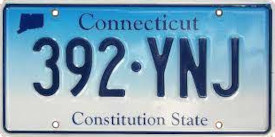
\includegraphics[height=.7in]{images/CTPlate1.jpeg}\hspace{.25in}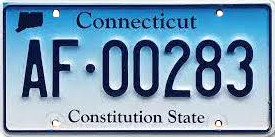
\includegraphics[height=.7in]{images/CTPlate2.jpeg}\hspace{.25in}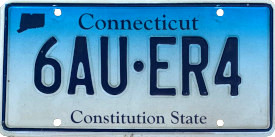
\includegraphics[height=.7in]{images/CTPlate3.jpg}
\end{center}

\item \textbf{When Order Does Not Matter:} Your local ice cream shop offers two types of cones: sugar and waffle. Sugar cones can hold up to two scoops of ice cream; waffle cones can hold up to three scoops of ice cream. Four flavors are available: chocolate, vanilla, strawberry, and rocky road. Assume that the order the scoops that come on the ice cream DOES NOT matter (e.g. two scoops with vanilla on top of chocolate is the same as two scoops with chocolate on top of vanilla).
\begin{enumerate}
  \item Explain why you cannot use the fundamental counting principle to solve this problem.
  
 \item Create an effective and organized way to list all the possible orders, and use it to list them.
 
 \item How many possible orders are there? 
\end{enumerate}

\item \textbf{Rhythms:}
 \begin{center}
    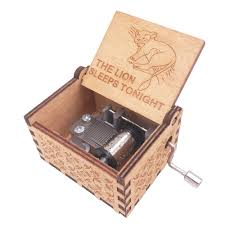
\includegraphics[height=2in]{images/MusicBox.jpeg}
\end{center}
 A music box like the one shown above contains a wheel the rotates around to play the music, so once the wheel has made a full revolution it repeats the same music over. Also since the crank determines how long the music is played the music could start and stop at any point along the wheel. If we only consider rhythm then the two four count rhythms 1100 and 0011 would be considered the same when put on a music box wheel. 
 \begin{enumerate}
 \item In class we created a list of all four count rhythms (there are 16 of them!) Group the ones that produce the same music box wheel together and determine how many music box wheel rhythms exist on four counts. Note: even though it wouldn't make any sound at all, count the "broken" music box wheel 0000 (four rests).
 \item Find how many different bracelets you can make with four beads if you only have two different colors of beads.
 \item Explain the connection between the four-bead bracelets and the four-count music boxes. Why are there the same number of each?
 \item Pick a rhythm on 8 counts that you like, and record yourself playing it on your instrument of choice (bells, guitar, drum, clapping, stomping your feet, etc.) three times over. You can use your phone's sound recorder. Write the rhythm using zeros and ones and say why you like it.
 \item BONUS! Find how many music box wheel rhythms there are on eight counts. (Hint: find the answer for small numbers like three counts, four counts, and five counts to come up with a method for tackling the larger problem.)
 \end{enumerate}
 \Instr{  Generalization is a difficult problem. There is no obvious pattern. See the following table.\par
 \begin{tabular}{c|c|c|c|c|c|c|c|c|c}
     counts & 0 & 1 & 2 & 3 & 4 & 5 & 6  & 7  & 8 \\\hline
     wheels & 1 & 2 & 3 & 4 & 6 & 8 & 14 & 20 & 36
 \end{tabular}\par
 See \href{https://oeis.org/A000031}{https://oeis.org/A000031}}
\end{enumerate}

\wbnewpage
%%%%%%%%%%%%%%%%%%%%%%%%%%%%%%%%%%%%%%%%
%%%%%%%%%  New Section  %%%%%%%%%%%%%%%%
%%%%%%%%%%%%%%%%%%%%%%%%%%%%%%%%%%%%%%%%
\section{Additional Exercises}

\begin{enumerate}
\item The Cuddle Toy factory makes $3$ different types of fluffy animals, each with its choices of add-ons: the turtle, the bunny, and the kitten. 
\begin{enumerate}
\item The turtle and bunny can each come with any number of the following: a top hat, a cane, and a monocle. The kitten and turtle have a choice of any number of the following: overalls, scarf, a shirt, and shoes. All three animals are available in one of the following three colors: blue, red, or green. 
%Construct the tree diagram to count the number of different fluffy animals that can be constructed by the Cuddle Love factory. 
How many different types of fluffy animals are there?
%</chap1:exercises:cuddleLove>

\Instr{ 
There are\\
$2\; (\text{overalls})\times 2\;(\text{scarf})\times 2\; (\text{shoes})\times 2 \;(\text{shirt})\times 3 \;(\text{color})=48$ different types of kittens and\\ 
$2\;(\text{overalls})\times 2\;(\text{scarf})\times 2\;(\text{top hat})\times 2\;(\text{cane})\times 2\;(\text{monocle})\times 2\;(\text{shirt})\times 2\;(\text{shoes})\times 3\;(\text{color})=384$ different types of turtles.\\ 
There are $2\;(\text{top hat})\times 2\;(\text{cane})\times 2\;(\text{monocle})\times 3\;(\text{color})=24$ different types of bunnies. So there are either $48+384+24=456$ different types of fluffy animals.
}

%<*chap1:exercises:cuddleLove2>
\item The color options are still the same for the three fluffy animals. The turtle and bunny still can each come with any number of the following: a top hat, a cane, and a monocle. The kitten and turtle are now only allowed a choice of any number of the following: overalls, bell-bottoms, a shirt, and shoes. How many different types of fluffy animals are there?
%</chap1:exercises:cuddleLove2>

\Instr{ 
It would be silly if the kitten or turtle wore both the bell-bottoms and overalls at the same time. So we have to disallow this option. There are three choices for the pants: overalls, bell-bottoms, or neither. So the number of choices for the kittens is\\
$3\; (\text{pants})\times 2\; (\text{shoes})\times 2 \;(\text{shirt})\times 3 \;(\text{color})=36$\\ 
and for the turtles is\\
$3\;(\text{pants})\times 2\;(\text{top hat})\times 2\;(\text{cane})\times 2\;(\text{monocle})\times 2\;(\text{shirt})\times 2\;(\text{shoes})\times 3\;(\text{color})=288$.\\
There are still $24$ different types of bunnies. Thus there are $36+288+24=348$ different types of fluffy animals.
}

%<*chap1:exercises:bebopMan>
\end{enumerate}

\item The Bebop manufacturing company produces license plates consisting of the following in the order given: one lower-case letter, one upper-case letter, two digits ($0$ through $9$), and finally three letters that may be upper- or lower-case.  How many different license plates can Bebop make? If I am assigned a plate at random, what is the probability that it starts with ``aA1''?
%</chap1:exercises:bebopMan>

\Instr{  Notice that the choice for each character on the license plate is independent from the choice of each other character. So we can use the Fundamental Counting Principle and multiply the number of options for each character. There are $26$ lower-case letters, $26$ upper-case letters, and $10$ numbers to choose from for each of the characters with numbers only. So there are $26\times 26\times 10 \times 10 \times 52 \times 52\times 52= 9,505,100,800$ different ways a license plate can be made by Bebop.

For the second question, a license plate with ``aA1'' in the first three positions can have any of the available letters and/or numbers that each digit is allowed for the remaining positions. So there are $10\times 52\times 52\times 52=1,406,080$ and the probability of having such a plate is $\frac{1,406,080}{9,505,100,800}=0.0001479$.
}

%<*chap1:exercises:areaCodesA>
\item Originally area codes were made up of three numbers ($0$ through $9$) where the middle digit was either $0$ or $1$ and the first digit was non-zero. 
\begin{enumerate}
\item\label{areaCodesAa} In this way, how many different area codes were possible?
%</chap1:exercises:areaCodesA>

\Instr{  
Choosing a number for the first digit does not affect the number of choices we have for subsequent digits. The same is true for each pair of digits. So we may use the Fundamental Counting Principle. The first digit cannot be $0$ so there are $9$ possibilities to choose from. The second digit can only be $0$ or $1$ which gives $2$ possibilities for this digit. The last digit has no restrictions, so there are $10$ possibilities. Thus, the number of ways to form an area code at this time is $9\times 2 \times 10=180$.
}

%<*chap1:exercises:areaCodesB>
\item To avoid emergency contact numbers such as $911$ and $411$ no area code is allowed to end with consecutive $1$'s. How many different area codes were there if all area codes that end in $11$ were forbidden?
%</chap1:exercises:areaCodesB>

\Instr{ 
By using our solution from Question~{\normalfont\ref{areaCodesAa}}, all we need to do is find the number of forbidden numbers and subtract it from $180$ possible area codes. A forbidden configuration contains two consecutive $1$ at the end of the area code, so they would be of the form $?11$. Thus there are ten area codes of forbidden configurations of the form $?11$. So there are $180-9=171$ area codes of the specified form.
}
%<*chap1:exercises:endSteveDice>
\end{enumerate}

\item\label{steveDice} Steve rolls three differently colored $6$-sided dice. How many different ways can the dice land?
%</chap1:exercises:endSteveDice>

\Instr{  The students may think that because each die is $6$-sided there are only $6$ ways for the three $6$-sided dice to land. But by using their color we establish that rolling a $1$ on one of the die is not the same as rolling a $1$ on a different die. 

Fortunately, rolling one die does not affect the outcome on any other die. So rolling each die is independent of rolling the another die and we can use the Fundamental Counting Principle. Since there are $6$ ways for a $6$-sided die to land, there are $6\times 6\times 6=216$ ways for the three $6$-sided dice to land.
}

%<*chap1:exercises:steveDiceRound2>
\item Using the three dice in Question~{\normalfont\ref{steveDice}}, you want to know the number of ways the dice can be rolled so that exactly two of the dice show the same number. How many different ways can this happen? 
%</chap1:exercises:steveDiceRound2>

\Instr{  
There are $\binom{3}{2}=3$ ways to choose the two dice that show that same number and these two dice can come up with $6$ possible numbers. The remaining die would have $5$ possible choices for the last number.  Since each of these events is independent, there are $3\times 6\times 5=90$ ways three $6$-sided dice can be rolled so that exactly two of the dice show the same number. 

Alternatively, we could argue in the following manner. Suppose the three dice are colored red, white, and blue. 
We split this problem into three disjoint counting problems:
\begin{packedEnum}
\item the number of ways that the red die does not match the other two dice but the white and blue dice show the same number,
\item  the number of ways that the white die does not match the other two dice but the red and blue dice show the same number, and 
\item the number of ways that the blue die does not match the other two dice but the red and white dice show the same number.
\end{packedEnum}
By symmetry, it is clear that the number of ways is the same in each of these three cases. So suppose the red dice does not match the other two dice but the white and blue dice show the same number. There are $6$ ways that the white and blue dice can show the same number: two $1$'s, two $2$'s, two $3$'s, two $4$'s, two $5$'s, and two $6$'s. With this chosen there are $5$ remaining options for the red die. Remember that there are exactly two dice that are the same. So the number of ways to count the statement in (a) is $6\times 5=30$. Since statements (b) and (c) are identical, there are $30$ ways to count the number of ways the $3$ dice can land in the indicated way. So there are $30+30+30=90$ ways three $6$-sided dice can be rolled so that exactly two of the dice show the same number.
}



%<*perm:exercises:appMainDessertA>
\item A restaurant has $12$ appetizers, $13$ main courses, and $11$ desserts.
\begin{enumerate}
 \item How many ways can you order a three-course meal (you must choose $1$ appetizer, $1$ main course, and $1$ dessert for your meal)?
%</perm:exercises:appMainDessertA>

 \Instr{ 
 There are $12\times 13\times 11=1716$ ways to order a three-course meal.
 }

%<*perm:exercises:appMainDessertB>
\item What is the probability that my desert is tiramisu (one of the $11$ choices for dessert) if I choose my $3$ courses randomly?
%</perm:exercises:appMainDessertB>

 \Instr{ 
 The probability of choosing tiramisu is $\frac{12\times 13\times 1}{12\times 13\times 11}=\frac{1}{11}$.
 }
 
 \end{enumerate}
 
%<*chap1:exercises:4charPlates>
\item\label{4charPlates} A special license plate consists of $4$ characters. Each character is either a letter or a digit (there are $26$ letters and $10$ digits. How many $4$-character license plates can be made where characters can be repeated on each plate?
%</chap1:exercises:4charPlates>

\Instr{  
There are $36$ letters and numbers to choose from for the first character. Since repetition is allowed, the choice for each character is independent of the other characters and so we can use the Fundamental Counting Principle. Thus, there are $36\times 36\times 36\times 36=36^4=1,679,616$ different ways to manufacture this license plate.
}

%<*chap1:exercises:5charPlates>
\item Using the description of a license plate from Question~{\normalfont\ref{4charPlates}}, how many $5$-character license plates can be made if repetition is allowed?
%</chap1:exercises:5charPlates>

\Instr{  As stated in Question~{\normalfont\ref{4charPlates}} choosing the characters is an independent action and so we can apply the Fundamental Counting Principle. Thus there are $36^5=60,466,176$ different ways to construct a license plate with $5$-characters.
}

%<*chap1:exercises:carCompanyA>
\item A car company makes cars of $2$ different body styles (compact and station wagon), $6$ different colors (blue, orange, green, black, red, and white), and $3$ model types (standard, all wheel drive, and luxury package).
\begin{enumerate}
\item\label{howManyCars} How many different types of cars can be built?
%</chap1:exercises:carCompanyA>

\Instr{  Since each of the options for the car are independent of each other, we can use the Fundamental Counting Principle to see that there are $2\times 6\times 3=36$ different cars that can be built.}

%<*chap1:exercises:carCompanyC>
\item If I choose my car at random from all the possibilities, what is the probability that I get a black station wagon?
%</chap1:exercises:carCompanyC>

\Instr{ 
To determine the number of different black station wagons we could possibly choose, we see that we have only three options for the model: standard, all wheel drive, and luxury package. So the probability of choosing a black station wagon is $\frac{3}{36}=0.0833$. 
}

%<*chap1:exercises:carCompanyB>
\item\label{noBlack} How many different types of cars can be built if the station wagon cannot be made in black? 
%</chap1:exercises:carCompanyB>

\Instr{  Since the station wagon cannot be made in black, we cannot use the Fundamental Counting Principle. The choice of station wagon affects the number of color choices we have. But if we count the number of different cars that can be made given that the car is compact and then count the number of different cars that can be made given that the car is a station wagon, then we have two disjoint events, so by adding the counts of the numbers of each car type together we can find the number of different cars that can be built. 

Suppose the car is compact. There are $6$ different color options and $3$ different models that can be built. These choices are independent, so by the Fundamental Counting Principle, there are $6\times 3=18$ different compact cars that can be built. 

Suppose the car is a station wagon. Then there are $5$ different color options and $3$ different models that can be built. These choices are independent, so by the Fundamental Counting Principle, there are $5\times 3=15$ different station wagons that can be built. In all, there are $15+18=33$ different types of cars that can be built.
}

%<*chap1:exercises:20trueFalse>
\end{enumerate}

\item\label{20trueFalse} There are $20$ true or false questions on a quiz given in your History class. In how many different ways can a student answer the test?
%</chap1:exercises:20trueFalse>

\Instr{  There are two ways to interpret this problem: you must answer each question or you can leave some questions blank. In the first version, there are two possible ways to answer each question: true or false. So there are $2\times 2\times \cdots\times 2=2^{20}$ different ways to answer the quiz. In the second version, there are three possible ways to answer each question: true, false, or blank. So there are $3\times 3\times \cdots\times 3=3^{20}$ different ways to answer the quiz.}

%<*chap1:exercises:10trueFalseA>
\item\label{10trueFalseA} There are $10$ true or false questions on a quiz given in a History class.
\begin{enumerate}
 \item Consider two students to have answered the test differently if they disagree in at least one of their $10$ answers. How many different ways are there to answer the $10$ questions on the test?
%</chap1:exercises:10trueFalseA>
 
 \Instr{ 
 As we saw in Question~{\normalfont\ref{20trueFalse}}, there are two ways to interpret this problem: you must answer each question or you can leave some questions blank. The answers to each of these questions are $2\times2\times \cdots\times 2=2^{10}$ and $3\times 3\times\cdots\times 3=3^{10}$ different ways to answer the quiz respectively. 
 }
 
 %<*chap1:exercises:10trueFalseB>
 \item If the student just rolls a die to randomly answer each question, what is the probability the student will get $100\%$ on the test (i.e., get all questions correct)?
 %</chap1:exercises:10trueFalseB>
 
 \Instr{ 
 There is exactly one way to get $100\%$ on the test but, as said in Question~{\normalfont\ref{10trueFalseA}}, there are two ways to interpret this question. Consequently, there are two ways to interpret this question as well. Depending on whether you must fill in all answer or you may leave some questions blank, the probability of getting $100\%$ on the test is $\frac{1}{2^{10}}$ or $\frac{1}{3^{10}}$ respectively.
 }
 
%<*chap1:exercises:4digitEven>
 \end{enumerate}

\item\label{4digitEven} How many $4$-digit even numbers use only the numbers $1$, $2$, $3$, $4$, and $5$?
%</chap1:exercises:4digitEven>

\Instr{  
Since there are $4$ digits in this number and the choice of one digit does not affect the choice of another digit, we can use the Fundamental Counting Principle to count the number of ways to form a $4$-digit number as described. There are $5$ different numbers that can be chosen for each of the leftmost $3$ digits. But the units digit must be even, so only $2$ or $4$ can be placed in the units digit. This gives us a grand total of $5\times 5\times 5 \times 2=250$ different $4$-digit even numbers that contain the numbers $1$, $2$, $3$, $4$, and $5$.
}

%<*chap1:exercises:4digitOdd>
\item How many $4$-digit odd numbers use only the numbers $1$, $2$, $3$, $4$, and $5$?
%</chap1:exercises:4digitOdd>

\Instr{  
As seen in Question~{\normalfont\ref{4digitEven}} the choice of each digit is independent of the others, allowing us to use the Fundamental Counting Principle. Again, there are $5$ choices for the first $3$ digits but this time there are $3$ choices for the units digit: $1$, $3$, or $5$. So there are $5\times 5\times 5\times 3=375$ different $4$-digit odd numbers that contain the numbers $1$, $2$, $3$, $4$, and $5$.
}

%<*chap1:exercises:15dmv>
\item There are $15$ people in a line to get their license at the Department of Motor Vehicles. Alice and Bob are two of the people in this line. In how many ways can the line be formed such that Alice is ahead of Bob?
%</chap1:exercises:15dmv>

\Instr{  Unfortunately, the choice of Bob's location does affect the number of choices for Alice's position in the line making this a dependent problem. But we can break this problem up based on the location of Bob. If Bob is last in line, there are $14$ different positions Alice could reside. If Bob is second to last in line, there are now only $13$ different positions for Alice to choose from. In this manner, the number of options for Alice decrease as Bob gets closer to the front of the line. Since each position for Bob is disjoint from each other position, the answer can obtained by adding these numbers. So there are 
$$14+13+12+11+10+9+8+7+6+5+4+3+2+1=105$$ 
different ways for Alice and Bob to stand in line so that Alice is ahead of Bob.
}


%<*chap1:exercises:iceCreamTree2A>
\item Your local ice cream shop offers $2$ types of cones: sugar and waffle. Sugar cones can hold up to $2$ scoops of ice cream; waffle cones can hold up to $3$ scoops of ice cream. Two flavors are available: chocolate and vanilla. Assume that the order the scoops come on the ice cream DOES NOT matter.
\begin{enumerate}
 \item Draw a tree that lists all the possible orders.
 %</chap1:exercises:iceCreamTree2A>

 %% TODO: provide solution
 
 %<*chap1:exercises:iceCreamTree2B>
 \item How many possible orders are there altogether?
 %</chap1:exercises:iceCreamTree2B>
 
 \Instr{ 
 $5$ orders on sugar cone and $9$ orders on waffle cone are possible. So that is $14$ altogether.
 }
 
 %<*chap1:exercises:iceCreamTree2C>
 \item If I select an ice cream order at random, what is the probability that my ice cream is on a waffle cone?
 %</chap1:exercises:iceCreamTree2C>
 
 \Instr{ 
 The probability that my ice cream is on a waffle cone is $9/14$.
 }
 
 %<*chap1:exercises:endIceCreamTree2>
\end{enumerate}
%</chap1:exercises:endIceCreamTree2>



\item\label{9outof10Ex} Out of $10$ ice cream flavors, how many different ways can you choose $9$ of them?
%</perm:exercises:9outof10Ex>

\Instr{  The number of ways to choose $9$ objects out of $10$ possible objects is based on the concept of choose numbers; $\binom{n}{r}$. So there are $\binom{10}{9}=\frac{10!}{1!\times 9!}=10$ different ways to choose $9$ of the $10$ ice cream flavors. You could also realize that exactly one flavor must be omitted, and there are clearly $10$ choices for that omitted flavor.
}
	
%<*perm:exercises:200flavors>
\item Out of $200$ ice cream flavors, how many different ways can you choose $5$ of them?
%</perm:exercises:200flavors>

\Instr{  As in Question~{\normalfont\ref{9outof10Ex}} the order in which we choose the ice cream flavors does not matter. So there are $\binom{200}{5}=\frac{200!}{195!\times 5!} =2,535,650,040$ different ice cream flavors.
Students may also answer by counting the number of letter codes with exactly $5$ $Y$'s (Yes, I want that flavor) and $195$ $N$'s; again this is $200!/(195!\times 5!)$.
}

%<*perm:exercises:chairpersonStudentCouncil>
\item\label{chairpersonStudentCouncil} In a student council meeting, there are $10$ people and you need to decide who is the chairperson, vice-chairperson, treasurer, and secretary. In how many different ways can this be done?
%</perm:exercises:chairpersonStudentCouncil>

\Instr{  It is clear that when $4$ people are chosen there is a order given to them based on who becomes the chairperson, the vice-chairperson, the treasurer, and the secretary. So we will use permutations to count the number of different ways these four positions can be counted. There are ${}_{10}P_4=10\times 9 \times 8\times 7=5040$ different ways to choose the chairperson, vice-chairperson, and treasurer from the $10$ people on the student council.}

%<*perm:exercises:studentCouncil2>
\item In a student council meeting, there are $10$ people and you need to choose $4$ people to be on a committee. In how many different ways can this be done?
%</perm:exercises:studentCouncil2>

\Instr{  In contrast to Question~{\normalfont\ref{chairpersonStudentCouncil}}, we do not care about the order of the $4$ people chosen. So there are $\binom{10}{4}=\frac{10!}{6!\times 4!}=210$ different ways to choose this committee.}

%<*perm:exercises:kingArthur>
\item King Arthur and his $9$ knights sit at the round table but one of the chairs is reserved for King Arthur. In how many ways can the $9$ knights seat themselves at the table?
%</perm:exercises:kingArthur>

\Instr{ 
By using King Arthur as the starting point, it makes counting the number of ways to arrange the knights around the table much easier. To the right of King Arthur, there are $9$ people who could sit in this chair. If a person sits in this chair, there are $8$ people remaining who can sit in the chair $2$ to the right of King Arthur. Every subsequent chair has one fewer person who could possibly sit in it. So there are $9\times 8 \times 7\times 6\times 5\times 4 \times 3 \times 2 \times 1=362,880$ different ways to seat the $9$ knights at the round table.
}

%<*perm:exercises:52cards>
\item In how many different ways can a deck of $52$ cards be arranged so that cards of the same suit are together? (Each of the cards falls into one of $4$ suits, and there are $13$ cards in each suit.)
%</perm:exercises:52cards>

\Instr{  
There are $2$ independent parts to this problem: the number of ways to arrange the suits and the number of ways to arrange the $13$ cards for each suit. Since the order matters and there are $4$ suits that all need a position, the number of ways to arrange the suits is ${}_4P_1=4!$ The number of ways to arrange the $13$ cards of each suit is a permutation problem as well. We have $13$ cards that can be placed into this first position, $12$ cards that can be placed into the next position, and so on. In all, there are $13!$ ways to arrange $13$ cards in each of the four suits. So there are $4!\times 13!\times 13!\times 13!\times 13!$ ways to arrange the a deck of cards to that cards of the same suit are together. 
}

%<*perm:exercises:end52cards2>
\item In how many different ways can you be dealt $5$ cards from a deck of $52$ cards?
%</perm:exercises:end52cards2>

\Instr{ 
This is a classic example of counting where order does not matter. There are $\binom{52}{5}=2,598,960$ ways to be dealt $5$ cards. 
}



%<*perm:exercises:endAppMainDessert>
\end{enumerate}
%</perm:exercises:endAppMainDessert>

%<*chap1:exercises:end>
%\end{enumerate}
%</chap1:exercises:end>

%<*chap1:exercises:endBowlIcecream>
%\end{enumerate}
%</chap1:exercises:endBowlIcecream>
